\documentclass[a4paper,10pt, twoside]{report}
\usepackage[utf8]{inputenc}
\usepackage[T1]{fontenc}
\usepackage{titlesec, blindtext, color}
\usepackage{setspace}
\usepackage{footnote}

\usepackage[export]{adjustbox}
\usepackage{array}
\usepackage{color, colortbl}
\usepackage{listings}
\usepackage{xcolor}

\usepackage{float}
\usepackage{fancyhdr}
\usepackage{fancyvrb}
\usepackage{graphicx}
\usepackage[top=2cm, bottom=3cm, left=2.5cm, right=2.5cm]{geometry}

\usepackage[french]{babel}

\usepackage[hidelinks]{hyperref}

% page style
\pagestyle{fancy}
\setlength{\headheight}{49pt}
\setlength{\footskip}{17pt}

% header
\fancyhead[R]{
\includegraphics[width=5cm]{logo_sciences.png}}
\fancyhead[L]{
\includegraphics[width=5cm]{logo_arksens.png}}

% footer
\fancyfoot[C]{Rapport de stage --- Master 2 FSIL\\Ludovic Lubeigt}
\fancyfoot[RO, LE] {\thepage}

% colors
\definecolor{gray73}{gray}{0.73}
\definecolor{arkred}{rgb}{0.592, 0.145, 0.168}
\colorlet{punct}{red!60!black}
\definecolor{background}{HTML}{EEEEEE}
\definecolor{delim}{RGB}{20,105,176}
\colorlet{numb}{magenta!60!black}

% commands
\newcommand{\hsp}{\hspace{20pt}}
\titleformat{\chapter}[hang]{\Huge\bfseries}
{\thechapter\hsp\textcolor{gray73}{|}\hsp}{0pt}{\Huge\bfseries}
\titleformat*{\section}{\LARGE\bfseries}
\titleformat*{\subsection}{\Large\bfseries}
\titleformat{\subsubsection}{\large\bfseries}{}{}
{\refstepcounter{subsubsection}~\thesubsubsection~}
\titleformat{\paragraph}{\bfseries\itshape}{}{}{\\}

\graphicspath{{images/}}


\lstdefinelanguage{json}{
    basicstyle=\normalfont\ttfamily,
%     numbers=left,
    numberstyle=\scriptsize,
    stepnumber=1,
    numbersep=8pt,
    showstringspaces=false,
    breaklines=true,
    frame=single, % line
%     backgroundcolor=\color{background},
    literate=
     *{0}{{{\color{numb}0}}}{1}
      {1}{{{\color{numb}1}}}{1}
      {2}{{{\color{numb}2}}}{1}
      {3}{{{\color{numb}3}}}{1}
      {4}{{{\color{numb}4}}}{1}
      {5}{{{\color{numb}5}}}{1}
      {6}{{{\color{numb}6}}}{1}
      {7}{{{\color{numb}7}}}{1}
      {8}{{{\color{numb}8}}}{1}
      {9}{{{\color{numb}9}}}{1}
      {:}{{{\color{punct}{:}}}}{1}
      {,}{{{\color{punct}{,}}}}{1}
      {\{}{{{\color{delim}{\{}}}}{1}
      {\}}{{{\color{delim}{\}}}}}{1}
      {[}{{{\color{delim}{[}}}}{1}
      {]}{{{\color{delim}{]}}}}{1},
}

\setcounter{tocdepth}{2}

\begin{document}
\begin{spacing}{1.2}
 
% Page de garde
\begin{titlepage}
  \newgeometry{top=2cm, bottom=2cm, left=2cm, right=2cm}
  
  \begin{center}
    
\includegraphics[width=9cm]{logo_sciences.png}\\[2cm]
    
    \textsc{\bfseries\Large Rapport de stage\\[0.3cm]
    Master 2 -- Fiabilit\'e, S\'ecurit\'e et
    Int\'egration Logicielle\\[0.3cm]
        Parcours Fiabilit\'e et S\'ecurit\'e Informatique}\\[0.3cm]

    \rule{\linewidth}{1mm} \\[1cm]

    \textsc{\bfseries\huge Conception \&  d\'eveloppement syst\`eme de backup
    chiffr\'e et incr\'emental en C/C++}\\[1cm]

    \rule{\linewidth}{1mm}\\[1.5cm]

    \textsc{\huge Arksens Cyber Security}\\[2cm]
    
    \begin{figure}[H]
      \begin{minipage}[t]{8cm}
        \centering
        
\includegraphics[scale=0.50]{logo_adhara.png}
      \end{minipage}
      \begin{minipage}[t]{8cm}
        \centering
        
\includegraphics[width=7cm]{logo_arksens.png}
      \end{minipage}\\[1.3cm]
    \end{figure}
      
    \begin{minipage}{0.4\textwidth}
      \begin{flushleft} \large
        \emph{\bfseries Auteur :}\\
        Ludovic \textsc{Lubeigt}
      \end{flushleft}
    \end{minipage}
    \begin{minipage}{0.4\textwidth}
      \begin{flushright}
        \large \emph{\bfseries Tuteur Entreprise :}\\
        Ga\"etan \textsc{van Diemen}\\[0.2cm]
        \emph{\bfseries Enseignant :}\\
        Jean-Luc \textsc{Massat}
      \end{flushright}
    \end{minipage}\\[1.5cm]
      
    \large\emph{\bfseries Ann\'ee Universitaire :}\\
    2014 -- 2015

  \end{center}
\end{titlepage}

\begin{abstract}

Ce document pr\'esente le travail r\'ealis\'e lors du stage de fin d'\'etude
\`a Arksens Ltd. \`a l'\^ile Maurice entre le premier avril 2015 et le 25
septembre 2015 dans le cadre du Master 2 Fiabilit\'e et S\'ecurit\'e
Informatique \`a l'Universit\'e d'Aix-Marseille.

Le rapport est d\'ecoup\'e en deux parties. Une premi\`ere servant de rapport
de synth\`ese et pr\'esentant l'entreprise, le sujet de stage, le
travail effectu\'e de m\^eme que l'environnement de travail et les \'eventuelles
difficult\'es rencontr\'ees.
La seconde partie apporte un aspect technique au rapport et permet de 
pr\'esenter le travail r\'ealis\'e plus en d\'etail.
\end{abstract}

\newpage
\hfill
\section*{Remerciements}
Je tiens tout d'abord \`a remercier l'\'equipe p\'edagogique de la facult\'e des
sciences de l'universit\'e d'Aix-Marseille qui m'a permis d'avoir les
connaissances et les aptitudes n\'ecessaires au bon d\'eroulement de ce stage.

Je remercie \'egalement la soci\'et\'e Arksens pour m'avoir permis de faire mon
stage chez eux. Tout particuli\`erement, je remercie David Terranova et Ga\"etan
van Diemen qui m'ont accueilli \`a l'\^ile Maurice et suivi au jour le jour
durant ces six mois, mais \'egalement Micha\"el Colaone et le reste de
l'\'equipe pour l'accueil et la bonne ambiance au sein de l'entreprise.

Enfin je remercie toutes les personnes que je peux oublier mais qui m'ont
aid\'e, dans l'\'ecriture de ce rapport, dans le cadre du stage ou qui m'ont
tout simplement fait d\'ecouvrir l'\^ile Maurice.

Je tiens tout particuli\`erement \`a remercier Sir Daniel Brands of House Brands,
the first of His Name, King of the Dutch, King of the flatlands and the first
Men, Breaker of Cars and Father of the Bikers.

\hfill
\tableofcontents
\thispagestyle{fancy}

\chapter*{Introduction}
\thispagestyle{fancy}
Dans le cadre du Master professionnel \textit{Fiabilit\'e, S\'ecurit\'e et
Int\'egration logicielle}, parcours \textit{Fiabilit\'e et S\'ecurit\'e
Informatique} \`a l'\textit{Universit\'e d'Aix-Marseille}, un stage de fin
d'\'etude doit \^etre effectu\'e en entreprise pour valider les acquis et
rentrer dans le monde professionnel.

J'ai r\'ealis\'e ce stage entre le 1\up{er} avril et le 25 septembre 2015, soit
une p\'eriode de six mois, dans l'entreprise \textit{Adhara Cyber Security},
renomm\'ee \textit{Arksens} au 1\up{er} juillet.

Ce stage fut donc l'occasion pour moi de mettre en pratique mes connaissances,
acquises tout au long de mon parcours universitaire, dans un environnement
professionnel et de m'en servir pour mener au mieux la mission qui m'a
\'et\'e confi\'ee. Ma mission, durant ce stage, a \'et\'e de concevoir et
d\'ev\'elopper un syst\`eme de backup incr\'ementale et s\'ecuris\'e, offrant
une encryption en local des donn\'ees des utilisateurs. J'ai ainsi proc\'ed\'e
\`a la r\'edaction du plan de d\'eveloppement puis \`a l'impl\'ementation de
celui-ci, et j'ai ainsi particip\'e au processus de cr\'eation, jusqu'\`a un
stade avanc\'e, de ce qui peut \^etre qualifi\'e de gros projet.

Ce rapport pr\'esente donc le d\'eroulement du stage ainsi que le travail
accompli au sein de l'entreprise durant ces six mois.


\chapter{Rapport de synth\`ese}
\thispagestyle{fancy}
\label{rapportSynthese}
\section{Pr\'esentation de l'entreprise}
Cr\'e\'ee en 2013 sous le nom d'\textit{Adhara Cyber Security} avant
d'\^etre renomm\'ee \textit{Arksens} au 1\up{er} juillet 2015, l'entreprise 
dans laquelle j'ai effectu\'e mon stage est sp\'ecialis\'ee en s\'ecurit\'e
informatique. L'entreprise se d\'eveloppe sur trois continents gr\^ace \`a une
approche novatrice et r\'epondant aux besoins des entreprises et
administrations de toutes tailles.

Le changement de nom a fait suite \`a une \'evolution des clients puisque
l'entreprise, bien que principalement prestataire de service pour des PME
s'est ouverte aux entreprises de taille plus importante. Revoyant leur
strat\'egie de commercialisation et de communication, l'entreprise se devait
donc de changer de nom.

\subsection{Pr\'esence dans le monde}
Aujourd'hui \textit{Arksens} est donc pr\'esent dans trois pays chacun sur
un continent diff\'erent (voir figure~\ref{mapArksens}) offrant ainsi aux
utilisateurs un service de proximit\'e :
\begin{itemize}
  \item Abu Dhabi aux \'Emirats Arabes Unis pour les activit\'es au Moyen
  Orient.
  \item Pamplemousses à l’\^ile Maurice pour les activit\'es africaines.
  \item Paris en France pour les activit\'es européennes.
\end{itemize}

\begin{figure}[h!]
  \centering
  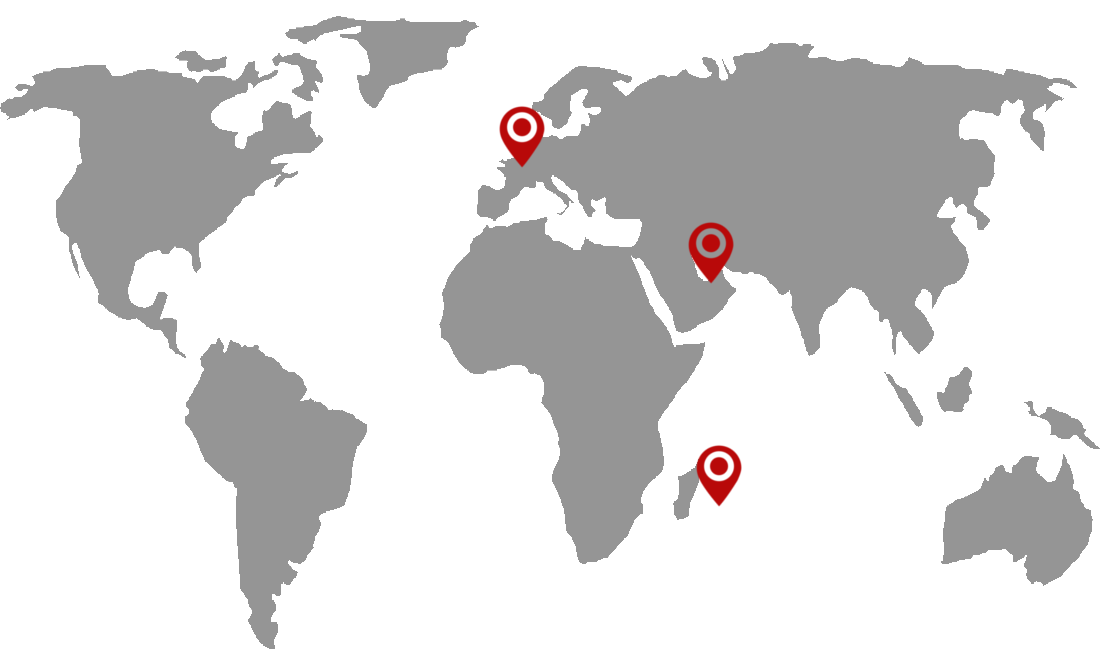
\includegraphics[scale=0.30]{map_arksens.png}
  \caption{\label{mapArksens} O\`u trouver Arksens}
\end{figure}
      
\subsection{Produits, solutions et offres}
\subsubsection{Les produits et solutions de s\'ecurit\'e}
\textit{Arksens} propose aux entreprises 6 produits et solutions autour de la
s\'ecurit\'e informatique. Une rapide description de ces produits se trouve
table~\ref{tabProduits} :
\begin{table}[h!]
  \centering
  \def\arraystretch{1.5}
  \setlength{\fboxsep}{13pt} % padding
  \setlength{\fboxrule}{0pt} % frame
  \begin{tabular}{m{6cm}m{6cm}}
   \rowcolor{arkred} 
    \arrayrulecolor{gray73}\hline
    \color{white} \textbf{Produit} & \color{white} \textbf{Description} \\
    
\includegraphics[width=5cm, fbox]{produits/mail.png} & Prot\'eger l'information
    transitant par les mails. H\'ebergement de serveur email s\'ecuris\'e dans
    un cloud d\'edi\'e.\\
    \hline
    
\includegraphics[width=5cm, fbox]{produits/whisper.png} & Communications voix
    et images s\'ecuris\'es et anonymes.\\
    \hline
    
\includegraphics[width=5cm, fbox]{produits/backup.png} & Syst\`eme de
    chiffrement et de sauvegarde des donn\'ees dans un cloud d\'edi\'e.\\
    \hline
    
\includegraphics[width=5cm, fbox]{produits/gateway.png} & S\'ecuriser et
    rendre anonyme la navigation sur internet.\\
    \hline
    
\includegraphics[width=5cm, fbox]{produits/endpoint.png} & S\'ecuriser les
    postes utilisateurs en locales. C'est une ligne de d\'efense pour palier
    \`a la diffusion d'\'eventuels logiciels malveillants (virus, chevaux de
    Troie, vers, logiciels espions,\ldots{}) sur les ordinateurs et les
    serveurs.\\
    \hline
    
\includegraphics[width=5cm, fbox]{produits/nomad.png} & S\'ecuriser les
    donn\'ees personnelles sur appareils mobiles.\\
    \hline
  \end{tabular}
  \caption{\label{tabProduits} Produits et solutions par \textit{Arksens}}
\end{table}

L'ensemble des produits et solutions propos\'es par l'entreprise sont d\'ecrit
de mani\`ere plus compl\`ete sur leur site web~\cite{refArksens}.

\subsubsection{Les offres de cloud}
L'entreprise propose \'egalement des offres autour du Cloud\footnote{
Exploitation de la puissance de calcul ou de stockage de serveurs distants
par l'interm\'ediaire d'un r\'eseau, g\'en\'eralement l'internet.}

\begin{itemize}
  \item Offre 1 - Pure cloud
  \noindent
  \begin{itemize}
    \item 100 \% des services sont h\'eberg\'es
    \item La gestion est assur\'ee par \textit{Arksens}
    \item Des fonctionnalit\'es suppl\'ementaires sont propos\'ees telles que
    l'h\'ebergement de fichiers ou de logiciels
  \end{itemize}
  \item Offre 2 - Hybrid cloud
  \noindent
  \begin{itemize}
    \item Un h\'ebergement local avec une ``box'' chifr\'ee et une
    r\'eplication sur le cloud \textit{Arksens}
    \item La gestion est assur\'ee par \textit{Arksens}
    \item Id\'eal pour les clients souhaitant une r\'eplication dans leurs
    locaux
  \end{itemize}
  \item Offre 3 - Private cloud
  \noindent
  \begin{itemize}
    \item Le cloud est pr\'esent uniquement chez le client dans une salle de
    serveurs ou dans un centre de donn\'ees
    \item La gestion est assur\'ee par \textit{Arksens}
    \item Id\'eal pour les clients souhaitant stocker l'ensemble des services
    et des donn\'ees localement (comme les banques, la d\'efense,
    l'audit\ldots{})
  \end{itemize}
\end{itemize}

Avec 3 offres de cloud comportant l'ensemble des solutions de s\'ecurit\'e
cité pr\'ec\'edemment, \textit{Arksens} peut répondre à l'ensemble des besoins
de ses clients actuels.

\subsection{L'id\'eologie de l'entreprise}
\subsubsection{La politique des centres de données}

Pour chaque service, \textit{Arksens} fournit le mat\'eriel (centres de
donn\'ees), le produit et le support qui va avec. Pour \^etre en mesure de
fournir les meilleurs services, elle poss\`ede une politique de s\'election des
centres de donn\'ees qu'elle utilise. Ci-dessous une liste repr\'esentant les
diff\'erents aspects les plus importants que doivent respecter les centres de
donn\'ees :

\begin{itemize}
  \item Uniquement des Tier IV (Haute disponibilit\'e\footnote{Mesure de
  performance. C'est le temps durant lequel le syst\`eme est op\'erationnel par
  rapport \`a sa dur\'ee totale d'exploitation} : 99,995 \%)
  \item Toutes les données sont chiffr\'ees sur les serveurs d\'edi\'es
  \item Les centres de donn\'ees doivent se situés dans des pays libres
  respectant le \textit{Patriot Act}~\cite{refPatriotAct}
\end{itemize}

De ce fait l'entreprise a actuellement des centres de donn\'ees en France
chez OVH~\cite{refOVH} qui lui conf\`ere en plus une solution contre les
attaques DDoS\footnote{Attaque par d\'eni de service. Le principe est d'envoyer
une multitude de requ\^ete depuis plusieurs sources diff\'erentes pour rendre
un service indisponible.} et en Suisse chez AlpineDC~\cite{refAlpineDC} dont la
l\'egislation est une des plus restrictive en mati\`ere de protection de
donn\'ees personnelles.

\subsubsection{La culture Open Source}

L'open source est une tradition dans l'entreprise. L'ensemble des
produits respectent les crit\`eres \'etablis par l'Open Source
Initiative~\cite{refOSI}, \`a savoir :

\begin{itemize}
  \item Possibilit\'e de redistribution
  \item Accès au code source
  \item Cr\'eation de travaux d\'eériv\'eés
\end{itemize}

Ce choix permet notamment d'accentuer la confiance avec les clients et
d'am\'eliorer le niveau de s\'ecurit\'e des produits gr\^ace aux avantages
suivants :

\begin{itemize}
  \item Logiciel ind\'ependant : aucune porte d\'erob\'ee
  (\textit{backdoor})\footnote{Fonctionnalit\'e inconnue de l'utilisateur
  l\'egitime et qui donne un acc\`es secret au logiciel} ne peut
  \^etre introduite par une organisation externe puisque les produits sont
  d\'evelopp\'es par \textit{Arksens} pour \textit{Arksens}
  \item Communaut\'e : l'acc\`es facile aux produits permet de cr\'eer une
  communaut\'e d'utilisateurs capable sur le long terme de proposer un
  support sur les produit d\'evelopp\'es, des am\'eliorations, mais aussi
  permet de d\'eceler des bogues
  \item Code source accessible : tout le monde a acc\`es au code source,
  rien n'est cach\'e, la cr\'edibilit\'e et la qualit\'e des produits est ainsi
  mise en avant
\end{itemize}

\subsection{\^Ile Maurice}
L'\^ile Maurice abrite es locaux accueillant le centre de recherche et
d\'eveloppement de l'entreprise. Les locaux se trouvent au Business Park de
Beau Plan (figure~\ref{beauPlan}) \`a Pamplemousses, ville situ\'ee au
nord-ouest de l'\^ile, \`a proximit\'e de Port Louis. C'est donc l\`a que
j'ai effectu\'e mon stage.

\begin{figure}[h!]
  \centering
  \includegraphics[width=15cm]{beau_plan_soir.jpg}
  \caption{\label{beauPlan} Beau Plan Business Park}
\end{figure}

L'\'equipe a beaucoup \'evolu\'ee entre mon arriv\'ee et mon d\'epart puisque
seulement trois personnes en plus du PDG, Micha\"el Colaone, \'etaient
pr\'esentes au 1\up{er} avril, date de d\'ebut du stage : David Terranova,
directeur des op\'erations, Ga\"etan van Diemen, chef de projet ainsi que
Daniel Brands, d\'eveloppeur web arriv\'e quelques jours auparavant.

L'\'equipe s'est agrandie par deux fois. D'abord \`a la mi-avril avec
l'arriv\'ee de deux autres stagiaire, Didier Mannone et
Yves Colin de Verdi\`ere, puis au 1\up{er} mai avec l'arriv\'ee d'Aymeric
Tabourin, ing\'enieur s\'ecurit\'e.

\`A mon d\'epart, une restructuration \'etait en cours et plusieurs changements
allait \^etre apport\'es au niveau de l'\'equipe en place avec notamment le
d\'epart de certains collaborateurs (licenciement, d\'emission ou tout
simplement fin de stage).

Ces changements montrent que la vie d'une startup peut rapidement \'evoluer,
que ce soit dans un sens ou dans l'autre. En l'espace de six mois seulement
une p\'eriode de recrutement s'en \'etait donc suivi d'une restructuration
importante impliquant le d\'epart de plusieurs employ\'es.

Durant mon stage dans l'entreprise, la pr\'esence de collaborateurs
N\'eerlandais et Mauriciens a permis la cr\'eation d'un environnement
international, bien que fortement francophone. Afin de pouvoir communiquer avec
l'ensemble des personnes de l'\'equipe, l'utilisation de l'anglais au quotidien
\'etait donc une n\'ecessit\'e.

L'int\'egration dans l'\'equipe s'est donc faite assez facilement et rapidement
et c'est ainsi dans une ambiance g\'en\'eralement bonne, bien que quelque peu
compliqu\'ee sur la fin d\^u \`a la restructuration de l'entreprise s'est
d\'eroul\'e ce stage de fin d'\'etude.

\section{Sujet de stage}
\subsection{Contexte}
L'entreprise \'etant encore jeune et de petite taille, plusieurs des services
existant \'etaient bas\'e sur des produits open source qui avaient \'et\'e
int\'egr\'e au \textit{manager} (voir figure~\ref{managerFront}).

Ce \textit{manager} est un environnement web d\'evelopp\'e et maintenu par
\textit{Arksens}. Il permet aux utilisateurs de g\'erer les services auxquels
ils ont souscrit \`a partir d'un unique endroit, centralis\'e, et ainsi
faciliter l'utilisation de ces derniers.

\begin{figure}[h!]
  \centering
  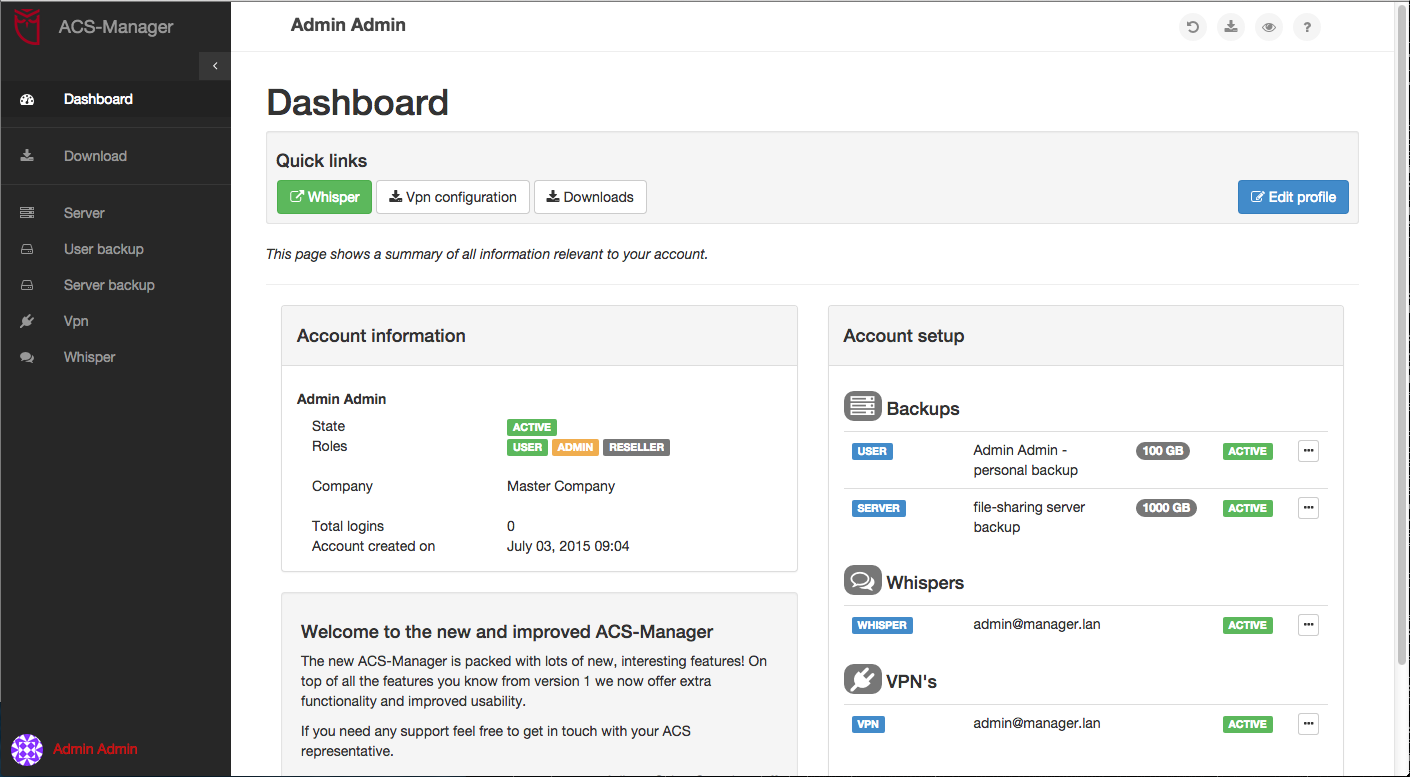
\includegraphics[width=15cm]{produits/manager.png}
  \caption{\label{managerFront} Page d'accueil du \textit{manager}}
\end{figure}

L'objectif de ce recrutement important \'etait pour l'entreprise de petit \`a
petit d\'evelopper ses propre solutions afin de proposer aux utilisateurs des
produits adapt\'es et r\'epondant \`a leurs besoins tout en minimisant
l'utilisation de logiciels tiers.

De plus les syst\`emes de backup ne sont souvent pas consid\'er\'es par les
entreprises avant qu'une perte de donn\'ees, plus ou moins importante,
ne survienne. Cons\'equences financi\`eres, temps pass\'e \`a reconstituer le
savoir \'evapor\'e ou encore impact sur la r\'eputation de l'entreprise ne sont
que des exemples de ce qui peut arriver dans une telle situation. Pour
pr\'evenir ce probl\`eme un syst\`eme de backup est non seulement n\'ecessaire
mais presque obligatoire.

Pour cela, \textit{Arksens} voulait offrir \`a ses clients un syst\`eme de
sauvegarde fiable, s\'ecuris\'e et optimis\'e afin de pouvoir \^etre
ex\'ecut\'e sur les ordinateurs les moins performants. De plus la prise en
compte de connexions internet pouvant \^etre parfois tr\`es lentes \'etait une
obligation. En particulier, une partie du march\'e vis\'e par \textit{Arksens}
se trouve en Afrique o\`u l'acc\`es \`a un internet rapide n'est pas toujours
aussi facile que ce qu'il peut y avoir en Europe.

C'est donc dans ce cadre que je suis arriv\'e et qu'il m'a \'et\'e demand\'e
de cr\'eer la prochaine g\'en\'eration de backup pour \textit{Arksens}.

\subsection{Le sujet}
Ma mission pour ce stage \'etait donc de faire la conception et le
d\'eveloppement d'un syst\`eme de backup incr\'emental et dont les donn\'ees
sauvegard\'ees sont chiffr\'ees en local, sur la machine client, avant d'\^etre
envoy\'ees sur des serveurs distant. Il me fallait donc d\'evelopper un
client/serveur multi-plate-forme, robuste et s\'ecuris\'e r\'epondant \`a
la probl\'ematique suivante : combiner le chiffrement local avec la sauvegarde
incr\'ementale.

De plus le programme devra \^etre \textit{multi-thread\'e} pour pouvoir
optimiser la sauvegarde des donn\'ees. Entre autre, cela permettra de chiffrer
des blocs, constituant les fichiers, tout en envoyant au serveur ceux d\'ej\`a
chiffr\'es.

Par ailleurs, allant \^etre un service propos\'e aux entreprises, il doit \^etre
pris en compte qu'un administrateur puisse g\'erer les diff\'erentes
sauvegardes ou \^etre inform\'e si un probl\`eme survient sur le poste d'un
employ\'e lors de l'utilisation du logiciel.

Enfin, un syst\`eme de quota devra \^etre mis en place. Ce syst\`eme permettant
aux entreprises de demander un plus ou moins grand quota selon la quantit\'e de
donn\'ees \`a sauvegarder. Celle-ci pouvant varier selon la taille ou la
fonction de l'entreprise, un quota permet une certaine flexibilit\'e.

Ce backup permettrait donc, au premier lancement, de sauvegarder l'ensemble
d'un ou plusieurs dossier. \`A partir de la seconde sauvegarde, il ne faudrait
n\'eanmoins sauvegarder que les changements sur les fichiers.

\`A mon arriv\'ee, David et Ga\"etan avait d\'ej\`a des id\'ees sur la
mani\`ere de r\'ealiser ce syst\`eme de sauvegarde, id\'ees que nous verrons
plus loin dans ce rapport. Et c'est \`a partir de celles-ci que j'ai pu
d\'emarrer mon travail, qui sera alors divis\'e en trois grandes phases :

\begin{itemize}
 \item Phase de documentation et de r\'eflexion sur la probl\'ematique
 \item Conception logicielle
 \item D\'eveloppement
\end{itemize}

La premi\`ere phase de documentation et de r\'eflexion consistait \`a
rechercher diff\'erentes solutions d\'ej\`a existantes et potentiellement
exploitable avant de proc\'eder \`a toute phase de conception.

La conception s'est faite en prenant en compte les contraintes existantes
et en se basant sur un travail de r\'eflexion d\'ej\`a effectu\'e par David et
Ga\"etan avant mon arriv\'ee.

Enfin, en ce qui concerne le d\'eveloppement, une des contraintes que j'avais
\'etait d'utiliser le C++ et de d\'evelopper de mani\`ere orient\'e objet tout
en faisant en sorte que le code puisse \^etre robuste, lisible, testable, et
donc facilement maintenable. De plus les librairies et framework utilis\'es
devaient \^etre sous licence libre afin d'\^etre en droit de publier l'ouvrage
sous licence libre.

Pour mener cette mission \`a bien, il avait \'et\'e d\'ecid\'e qu'une r\'eunion
hebdomadaire devait \^etre r\'ealis\'ee afin que David et Ga\"etan puissent
suivre l'avancement du projet mais aussi pour voir le travail effectu\'e la
semaine pr\'ec\'edente, essayer de r\'esoudre tout probl\`eme qui aurait pu
survenir et planifier la semaine suivante.
C'est en tout cas dans cette optique l\`a que nous avions commenc\'e. Dans les
fait, le retour des clients de l'entreprise lors de mises \`a jour des produits
ou des r\'eunions avec de potentiels futurs clients pouvaient prendre la
priorit\'e et ainsi retarder ou annuler les r\'eunions hebdomadaire.

\section{D\'eroulement du stage}
Avant de commencer le projet en lui-m\^eme, David et Ga\"etan m'ont fait part
de leur r\'eflexion sur le possible fonctionnement du syst\`eme de sauvegarde.

\begin{figure}[h!]
    \hspace{-4.5em}
    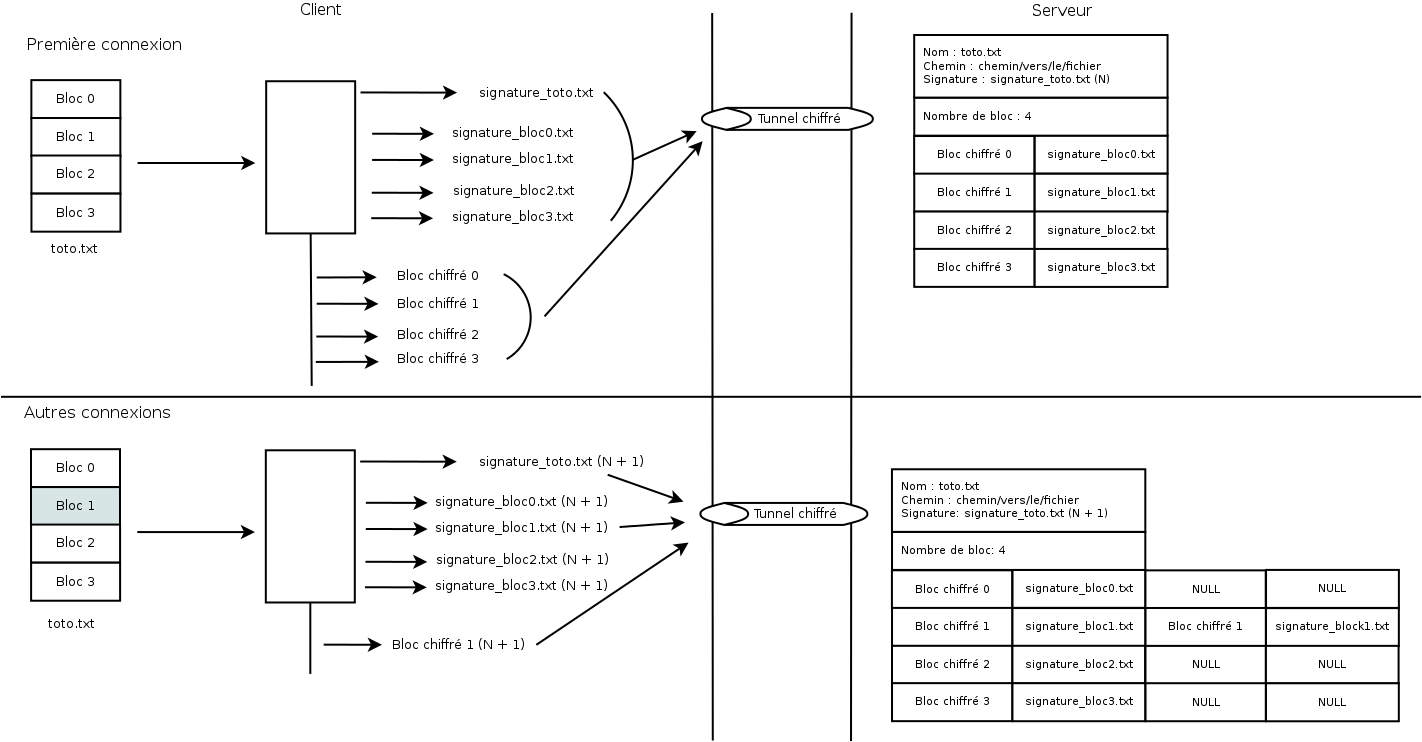
\includegraphics[width=19cm]{algo/schemaInitial.png}
    \caption{\label{schemaInitial} Sch\'ema initial du fonctionnement du backup}
\end{figure}

Le syst\`eme a deux comportement diff\'erent lors de la sauvegarde d'un fichier.
D'abord pour la premi\`ere connexion, o\`u une sauvegarde int\'egrale est
n\'ecessaire, puis lors des connexions suivantes o\`u seulement les
modifications doivent \^etre envoy\'ees.

Dans le premier cas, le fichier est d\'ecoup\'e en blocs de taille \'egale
avant d'\^etre chiffr\'e puis envoy\'e accompagn\'e des signatures calcul\'es
pour chaque bloc ainsi que pour le fichier en lui m\^eme. Les signatures
permettant de v\'erifier l'int\'egrit\'e des fichiers.

Le second cas est un peu plus complexe et d\'ecrit comme suit :
\begin{itemize}
 \item Calculer \textit{signature\_toto.txt} (\(N + 1\))
 \item T\'el\'echager \textit{signature\_toto.txt} (\(N\))
 \item Comparer les deux signatures : si elles ne sont pas diff\'erentes, les
 fichiers n'ont pas \`a \^etre compar\'e et on peut passer au fichier suivant
 sinon on continue
 \item D\'ecouper toto en bloc
 \item Calculer la signature de chaque bloc (\(N + 1\))
 \item T\'el\'echarger la signature de chaque bloc (\(N\))
 \item Comparer les chaque signatures
 \item Pour chaque signature diff\'erente, envoyer sur le serveur le bloc
 chiffr\'e correspondant accompagn\'e de sa signature (\(N + 1\))
\end{itemize}

Dans le cas de la figure~\ref{schemaInitial}, le bloc 1 \'etant modifi\'e, sa
signature, \`a \(N + 1\), ne correspond pas \`a la signature pr\'ec\'edemment
calcul\'ee (\(N\)). Le bloc est donc chiffr\'e avant d'\^etre envoy\'e sur le
serveur avec sa signature \textit{signature\_bloc1.txt}.

\paragraph{}
L'id\'ee, bien qu'int\'eressante dans un premier temps, ne peut \^etre
appliqu\'ee que dans un cas tr\`es particulier de fonctionnement et ne peut
donc pas \^etre utilis\'e en tant que tel :
\begin{itemize}
 \item Si les modifications n'affecte pas la taille d'un bloc et donc
 uniquement son contenu et que l'ordre des blocs est rest\'e inchang\'e
\end{itemize}

Pour tout les autres cas (ajout, suppression, d\'eplacement de tout ou partie
d'un bloc, etc.), l'algorithme ne pourrait pas fonctionner. Pour palier \`a
cela, j'ai donc d\^u imaginer un algorithme r\'epondant \`a la probl\'ematique
et fonctionnant dans tout les cas possible.

\subsection{Travail de recherche}
\label{secTravailRecherche}
\subsubsection{Documentation}
Mon travail de recherche s'est fait \`a partir d'une liste de mots-cl\'es qui
m'a \'et\'e donn\'e afin que l'on parle tous le m\^eme langage. Entre autre,
certaines d\'efinitions li\'ees au backup et au chiffrement :
\begin{itemize}
 \item Backup incr\'emental\footnote{Sauvegarde de fichiers dont le principe est
 d'envoyer uniquement les fichiers modifi\'es depuis la derni\`ere sauvegarde
 effectu\'ee}
 \item Backup diff\'erentiel\footnote{Sauvegarde de fichiers dont le principe
 est d'envoyer uniquement les fichiers modifi\'es depuis la derni\`ere
 sauvegarde compl\`ete effectu\'ee}
 \item Transchiffrement\footnote{Technique consistant, lors d'un changement
 de cl\'e de chiffrement, \`a d\'echiffrer l'ensemble des donn\'ees avec la
 pr\'ec\'edente cl\'e puis \`a les re-chiffrer avec la nouvelle}
\end{itemize}

Mais aussi des logiciels d\'ej\`a existant, de backup ou de synchronisation de
fichiers et \`a partir desquels il pouvait \^etre int\'eressant de s'inspirer :
\begin{itemize}
 \item Syncthing~\cite{refSyncthing}
 \item rsync~\cite{refRsync}
\end{itemize}

\paragraph{Syncthing}
\textit{Syncthing} est un logiciel permettant la synchronisation des donn\'ees
entre plusieurs appareils au travers d'une communication s\'ecuris\'ee via TLS.
Les donn\'ees n'\'etant jamais stock\'ees sur un serveur tiers, uniquement les
diff\'erents ordinateurs utilis\'es y ont donc acc\`es.

L'aspect int\'eressant de \textit{Syncthing} est pour nous le protocole de
communication, qui a \'et\'e cr\'ee \`a l'occasion : Block Exchange Protocol
(BEP)~\cite{refBEP}. Ce protocole sous Creative Commons~\cite{refCC4.0}, est
donc une bonne source d'inspiration afin de faire la liaison entre notre client
et notre serveur.

\paragraph{rsync}
\textit{rsync} est un programme de transfert de fichiers pour les syst\`emes
Unix. Le c\oe ur du programme est son algorithme sch\'ematis\'e
figure~\ref{rsyncAlgo} :
\textit{\flqq rsync algorithm \frqq}~\cite{refRsyncAlgo}.

\begin{figure}[h!]
    \centering
    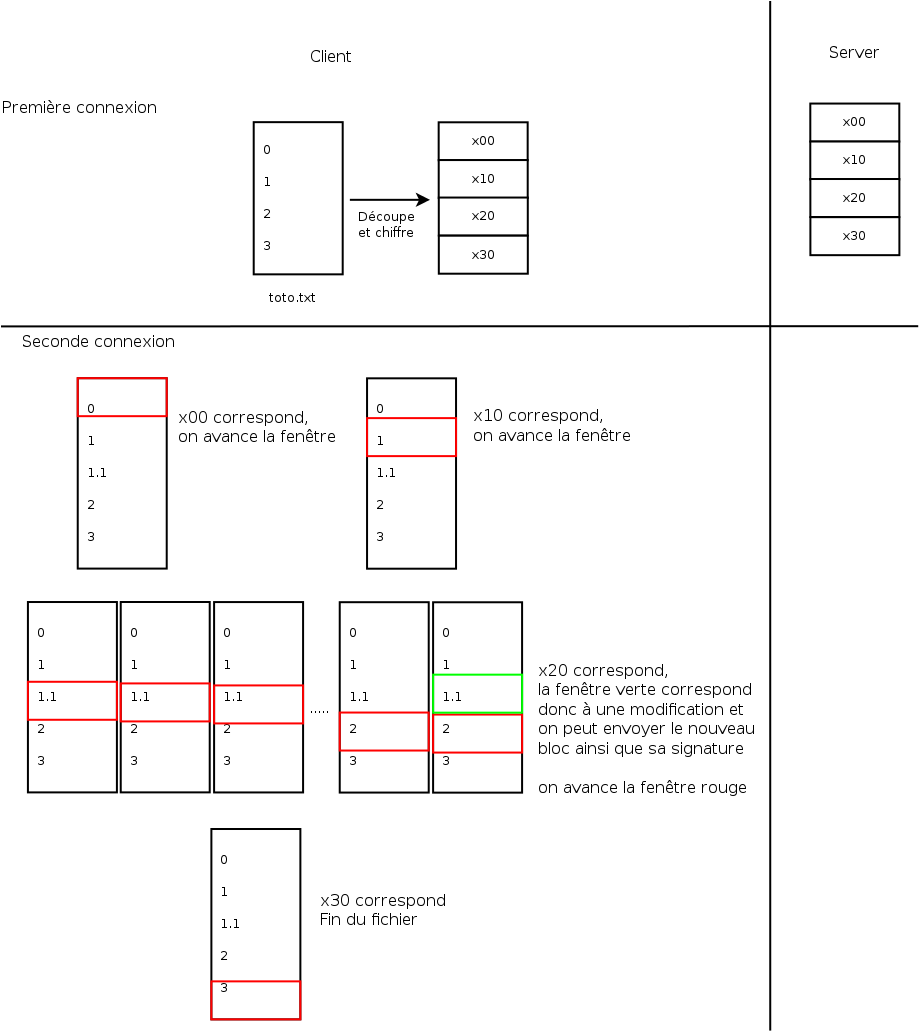
\includegraphics[width=15cm]{algo/rsyncalgo.png}
    \caption{\label{rsyncAlgo} Sch\'ema montrant bri\`evement
    l'algorithme \textit{rsync}}
\end{figure}

Celui-ci va d\'ecouper un fichier en plusieurs blocs de taille identique avant
de calculer, pour chacun, un \texttt{checksum} ainsi qu'un \texttt{hash}.

Pour n'envoyer que les parties modifi\'ees d'un ficher, l'algorithme va cr\'eer
une fen\^etre de la taille des blocs. Celle-ci va parcourir l'int\'egralit\'e
du fichier octet par octet.

Pour chaque position de la fen\^etre, le \texttt{checksum} --- rapide \`a
calculer mais dont le risque de collision est \'elev\'e --- est calcul\'e et
compar\'e au \texttt{checksum} d\'ej\`a calcul\'e au pr\'ec\'edent backup de
chaque bloc composant le fichier. Si un \textit{checksum} correspond, le
\texttt{hash} --- plus lent \`a calculer mais un risque de collision beaucoup
plus faible, selon l'algorithme utilis\'e --- du bloc correspondant est alors
comparer. Si celui-ci est identique, la fen\^etre correspond \`a un bloc non
modifi\'e du fichier.

Ainsi, tout ce qui pr\'ec\`ede la fen\^etre, et jusqu'au pr\'ec\'edent bloc
trouv\'e, correspondant \`a une partie du fichier modifi\'ee
(ajout/modification/suppression) et doit donc \^etre synchronis\'e.

C'est en grande partie cet algorithme qui m'a permis d'en trouver me permettant
de r\'epondre \`a ma probl\'ematique. Probl\'ematique \`a la fois similaire au
probl\`eme de \textit{rsync} puisqu'il fallait comparer deux fichiers distant
pour n'envoyer les changements mais diff\'erent dans la mesure o\`u il n'est
pas possible dans mon cas de maintenir une liste de bloc de m\^eme taille au
del\`a du premier backup.

\subsubsection{R\'eflexion}
Une fois cette phase de documentation r\'ealis\'ee, il \'etait temps de trouver
un algorithme permettant d'identifier les parties d'un fichier ayant \'et\'e
modifi\'e depuis le pr\'ec\'edent backup. Pour ce faire, et comme indiqu\'e
dans la partie documentation, je me suis bas\'e sur l'algorithme \textit{rsync}
pour, petit \`a petit, cr\'eer un algorithme qui permettait de r\'epondre \`a ma
probl\'ematique.

\paragraph{Chiffrement homomorphe}
Dans un premier temps, j'ai \'etudi\'e la question de l'homomorphisme. Ce type
de chiffrement permet de r\'ealiser des op\'erations sur des fichiers chiffr\'es
et de retourner le r\'esultat chiffr\'e. Ceci permet de faire des op\'erations
sans avoir \`a conna\^itre le contenu d'un fichier.

\begin{itemize}
 \item \textbf{Fonctionnement :} Dans notre cas, il nous aurait permis de
 concatener sur le serveur l'ensemble des morceaux d'un fichier avant de le
 re-d\'ecouper en bloc de taille \'egale puis de calculer pour chacun le
 \texttt{checksum} ainsi que le \texttt{hash}. Ceci aurait permis d'utiliser
 directement l'algorithme \textit{rsync} pour identifier les modifications
 faites sur un fichier.

 \item \textbf{Avantage :} Consommation de ressource et temps de calcul
 r\'eduit sur la machine client.
 
 \item \textbf{Inconv\'enient :} En utilisant le chiffrement homomorphe, le
 plus gros du calcul se fait sur le serveur entre deux backup, et ceux pour
 chaque fichier de chaque utilisateur. Ce type de chiffrement est donc tr\`es
 demandeur de ressource du c\^ot\'e du serveur pour que le programme fonctionne
 correctement.

 \item \textbf{Probl\`eme :} Le chiffrement homomorphe est un domaine de
 recherche tr\`es prometteur mais pas encore assez avanc\'e pour pouvoir
 \^etre utilis\'e en production. De plus le temps de calcul est extr\^emement
 \'elev\'e. Cette solution ne peut donc pas \^etre utilis\'ee aujourd'hui mais
 pourra peut-\^etre un jour \^etre envisag\'ee dans une prochaine version du
backup.
\end{itemize}

\paragraph{rsync revisit\'e}
\'Etant donn\'e que les fichiers doivent \^etre chiffr\'es et d\'echiffr\'es
uniquement sur la machine h\^ote (le client), nous ne pouvons effectuer des
op\'erations sur ceux-ci du c\^ot\'e du serveur. Il fallait trouver un
algorithme qui permette de d'analyser un fichier en un temps fini. J'ai donc
d\'ecid\'e de baser mon travail sur le principe de fen\^etre glissante
utilis\'ee pour \textit{rsync}. Ne pouvant pas avoir des morceaux de fichier de
taille identique, il a fallu modifier l'algorithme pour prendre ceci en compte.
Ainsi avoir une fen\^etre dynamique semblait \^etre l'option \`a prendre.

\begin{itemize}
 \item \textbf{Fonctionnement :} L'algorithme utilise une fen\^etre dynamique,
 parcourant l'int\'egralit\'e du fichier et adaptant sa taille en fonction
 des longueurs des morceaux de fichier que nous avons.
 
 \item \textbf{Avantage :} Fait c\^ot\'e client, il n'y a pas une
 sur-utilisation des ressources serveurs qui est alors utilis\'e uniquement
 pour stocker les donn\'ees une fois chiffr\'ees.
 
 \item \textbf{Inconv\'enient :} Temps de calcul potentiellement grand,
 d\'ependant de la taille des fichiers \`a analyser ainsi que de ressources
 disponible sur la machine client.
\end{itemize}

C'est donc sur cette base que j'ai commenc\'e l'\'etape suivante. \'Etape 
consistant \`a \'ecrire un prototype permettant de v\'erifier la faisabilit\'e,
notamment en ce qui concerne le temps d'ex\'ecution du programme.

\subsubsection{Prototypage}
La v\'erification pratique de la th\'eorie \'etait n\'ecessaire avant de
pouvoir penser \`a la conception du produit. Pour cela, le passage par une
\'etape de prototypage semblait in\'evitable.

Dans ce cadre, j'ai \'ecrit l'algorithme en \textit{C++} afin de v\'erifier
le temps d'ex\'ecution de celui-ci. Plusieurs essais ont \'et\'e fait afin de
r\'eduire toujours plus la dur\'ee d'ex\'ecution de l'algorithme. C'est donc
principalement de l'optimisation, \`a la fois au niveau algorithmique et
qu'au niveau de l'\'ecriture du code en lui-m\^eme, que j'ai effectu\'e  au
cours de cette \'etape.

Plusieurs version ont donc vu le jour au cours de cette \'etape afin d'obtenir
un algorithme qui puisse \^etre utilisable pour le syst\`eme de backup. Dans
le cas \'ech\'eant il aurait fallu chercher un algorithme diff\'erent pour
atteindre notre objectif. N\'eanmoins cela n'a pas \'et\'e le cas. Le
prototype \'ecrit ayant permis de valider le fonctionnement de l'algorithme
trouv\'e, j'ai pu passer \`a l'\'etape suivante et commencer ainsi la
conception.
Plus de d\'etails sur ces diff\'erentes versions de l'algorithme peuvent \^etre
trouv\'es dans la partie~\nameref{rapportTechnique}.

\subsection{Conception}
\subsubsection{Un programme modulaire}
La conception a commenc\'e avec le d\'ecoupage du projet en diff\'erents
modules. Avant de penser \`a la partie serveur, c'est le client qui, dans un
premier temps, va \^etre la priorit\'e.

\begin{figure}[h!]
  \centering
  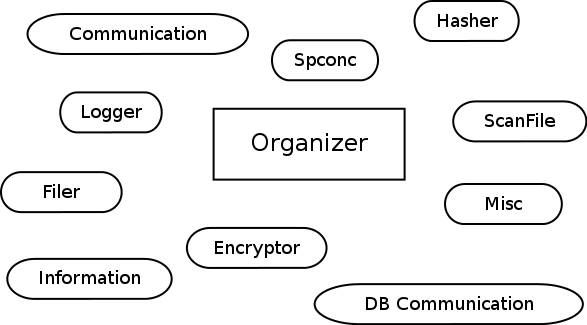
\includegraphics[scale=0.51]{softwareDesign/overviewModule.png}
  \caption{\label{overviewModule} Vue d'ensemble des modules}
\end{figure}

Pour celui-ci, dix modules vont \^etre utilis\'es autour d'un module central :
\begin{itemize}
  \item \textbf{organizer :} module central qui va cr\'eer plus ou moins de
  \textit{thread} et lancer les diff\'erents modules n\'ecessaires \`a la
  sauvegarde ou \`a la r\'ecup\'eration des donn\'ees.
  \item \textbf{information :} ce module contient les informations
  (m\'eta-informations) n\'ecessaires sur les morceaux de fichiers ainsi que
  sur les fichiers en eux-m\^eme.
  \item \textbf{filer :} ce module r\'ecup\`ere la liste des fichiers \`a
  partir du r\'epertoire d'entr\'ee. Il cr\'ee les objets correspondants
  (module information) et les transmets au module suivant.
  \item \textbf{spconc :} ce module coupe (\textit{split}) ou concat\`ene ce
  qui lui est envoy\'e selon qu'il s'agisse d'une sauvegarde ou d'une
  r\'ecup\'eration de donn\'ees.
  \item \textbf{scanFile :} dans le cas o\`u un fichier a d\'ej\`a \'et\'e
  sauvegard\'e, ce module va scanner l'int\'egralit\'e du fichier pour trouver
  les parties qui ont \'et\'e modifi\'ees et qui doivent \^etre chiffr\'ees et
  envoy\'ees au serveur.
  \item \textbf{hasher :} ce module fournit des fonction de hash permettant de
  v\'erifier l'int\'egralit\'e des fichiers.
  \item \textbf{encryptor :} ce module s'occupe du chiffrement et du
  d\'echiffrement des donn\'ees.
  \item \textbf{communication :} ce module s'occupe de la communication avec
  le serveur.
  \item \textbf{dbcomm :} ce module contient les fonctions utilis\'ees pour la
  communication avec la base de donn\'ees
  \item \textbf{misc :} ce module contient divers outils
  (\textit{miscellaneous}) pouvant \^etre utile dans le programme. Entre autre
  il contient le syst\`eme de notification permettant la communication entre
  les diff\'erents modules
  \item \textbf{logger :} ce module permet de garder une trace lors de
  l'ex\'ecution du programme, notamment utile lors du d\'eboguage ou si une
  erreur provoque l'arr\^et pr\'ematur\'e du programme.
\end{itemize}

\paragraph{}
L'utilisation de modules doit permettre une modification facile du programme,
sans avoir \`a modifier tout le code. Par exemple, pour changer un algorithme,
il ne doit donc \^etre n\'ecessaire que d'\'ecrire le code de celui-ci, sans
modifier celui en place, et de ne changer que la cr\'eation d'un objet \`a
partir du module en sp\'ecifiant un diff\'erent algorithme utilis\'e.

Un autre avantage de la programmation modulaire est la facilit\'e que cela
apporte pour maintenir le code efficacement.

Dans ce but, j'utiliserai et profiterai des sp\'ecificit\'es qu'offre la
programmation orient\'ee objet.

\subsubsection{Interaction entre modules}

L'utilisation de \textit{threads} pour ex\'ecuter les diff\'erents modules
complexifie l'interaction entre ceux-ci. Plusieurs modules sont utilis\'es
successivement pour pouvoir traiter un fichier, de la lecture depuis le disque
jusqu'\ \`a l'envoie des blocs, chiffr\'es, le constituant (dans le cas d'une
sauvegarde). Dans ce sens, les modules doivent communiquer entre eux. Un lien
est donc n\'ecessaire pour que deux \textit{threads} puisse s'envoyer les
donn\'ees li\'ees \`a un fichier.

\paragraph{Design pattern}
\subparagraph{Observer\\}
Pour faire ce lien, nous avons dans un premier temps pens\'e au design pattern
\textit{observer}, dont le principe est que lors du changement d'\'etat d'un
module, les autres module l'observant sont avertis et peuvent, ou non, agir en
cons\'equence. Cela donne \'egalement la possibilit\'e \`a un module d'envoyer
des informations en passant dans un certain \'etat \`a des moments cl\'es. Dans
notre cas, elles auraient correspondu aux m\'eta-donn\'ees d'un fichier,
accompagn\'e d'un \textit{pipe} servant de tunnel pour faire transiter le
fichier en lui-m\^eme d'un \textit{thread} \`a un autre.

Cette solution ne fut n\'eanmoins pas retenue puisqu'elle impliquait qu'un
module ait connaissances de celui \`a qui envoyer les informations. Ceci
n'\'etait pas voulu afin de laisser les modules aussi ind\'ependant que
possible.

\subparagraph{Event Notifier\\}
Pour palier \`a cela, un syst\`eme de notification a donc \'et\'e
impl\'ement\'e. Le principe de ce syst\`eme est relativement simple \`a
comprendre. On peut d'ailleurs trouver le m\^eme syst\`eme dans la vie de
tous les jours. Par exemple un journal publie r\'eguli\`erement des nouvelles
ayant un certain libell\'e (\flqq alertes\frqq, \flqq national\frqq, \flqq
sport\frqq, etc.). En face, il existe des utilisateurs qui peuvent, ou non,
s'inscrire \`a un ou plusieurs type de nouvelle. Ainsi, quelqu'un inscrit aux
nouvelles de type \flqq alertes\frqq va recevoir une notification lorsqu'une
nouvelle de ce type appara\^it.

Le principe utilis\'e dans notre cas est exactement le m\^eme : des modules
lancent des notifications que d'autres re\c{c}oivent s'ils se sont inscrits \`a
celles-ci.

Pour que cela fonctionne correctement, un centre de notification est
n\'ecessaire. Ainsi, et contrairement \`a un syst\`eme d'\flqq observer\frqq,
les modules n'ont pas \`a avoir connaissance les uns des autres puisque chacun
passe par ce centre.

Celui-ci est pr\'esent\'e figure~\ref{classDiagramNotif}. On retrouve le
centre de notification \textit{CNotificationService} qui g\`ere les
abonnements et les abonn\'es. Ce centre permet ainsi de les notifier les modules
ayant souscrit \`a un certain type de notification. Pour utiliser ce service,
il existe deux interfaces : \textit{ISubscriber} pour les abonn\'es et
\textit{INotifier} pour \'emettre les notifications. Ces interfaces sont donc
impl\'ement\'ee par les diff\'erents modules utilisant le syst\`eme de
notification.

\begin{figure}[h!]
  \hspace{-4.5em}
  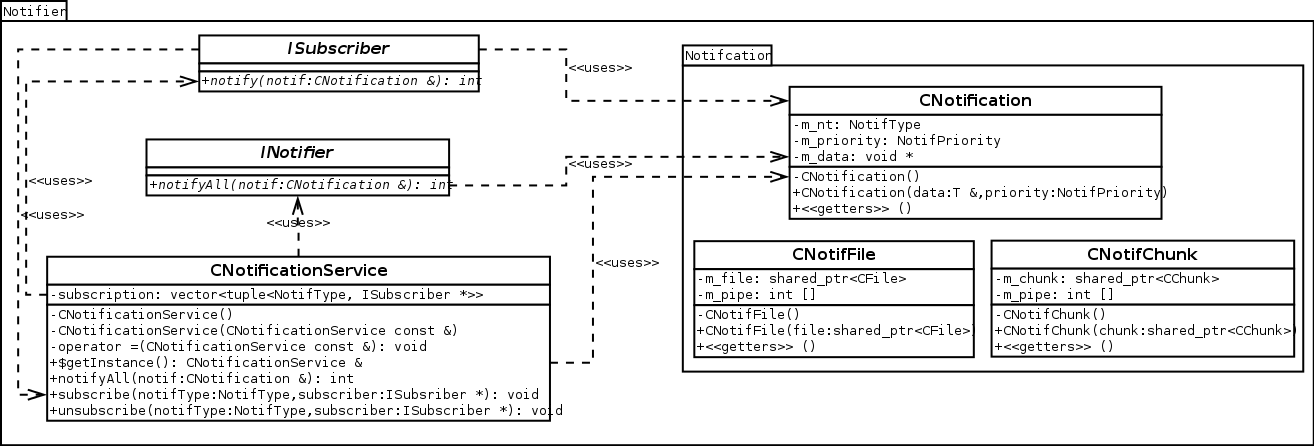
\includegraphics[width=19cm]{softwareDesign/classDiagramNotif.png}
  \caption{\label{classDiagramNotif} Diagramme de classe --- notifications}
\end{figure}

\paragraph{}
\begin{figure}[h!]
  \hspace{-1.5em}
  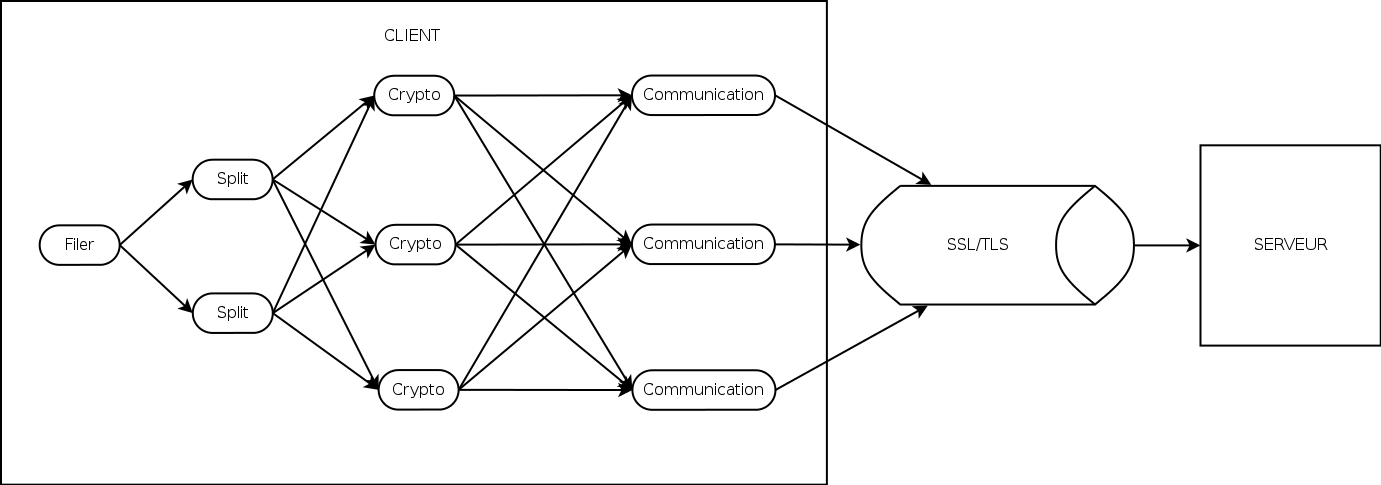
\includegraphics[width=17cm]{softwareDesign/moduleInteraction.png}
  \caption{\label{interactModule} Fonctionnement lors d'une premi\`ere
  sauvegarde}
\end{figure}

La figure~\ref{interactModule} montre comment le programme fonctionne dans le
cas d'une premi\`ere sauvegarde sur le serveur. Chaque noeud \`a l'int\'erieur
du client est un module exploitant un \textit{thread} diff\'erent. Ainsi
avons-nous :
\begin{itemize}
 \item une seule instance de \textit{Filer} est ex\'ecut\'ee. Le module
 communique avec une des instances libre du module \textit{Split}, i.e.~qui
 n'est pas d\'ej\`a en train de travailler sur un fichier
 \item \`A son tour, le module \textit{Split} communique avec n'importe quel
 \textit{thread} ex\'ecutant le module \textit{Crypto} en lui envoyant les
 donn\'ees \`a chiffrer.
 \item Enfin, celui-ci envoie les donn\'ees chiffr\'ees au module
 \textit{Communication} qui va simplement s'occuper de les envoyer sur le
 serveur.
\end{itemize}

\subsubsection{Base de donn\'ees}
\`A la fois du c\^ot\'e client et du c\^ot\'e serveur, l'utilisation d'une
base de donn\'ees semblait obligatoire afin de garder les m\'eta-donn\'ees
des fichiers sauvegard\'es mais \'egalement pouvoir garder en m\'emoire une
trace de chaque sauvegarde effectu\'ee. Cela donnerait la possibilit\'e
de restaurer n'importe quelle version d'un ou plusieurs fichier(s). En effet,
nous aurions ainsi dans l'ensemble des informations n\'ecessaires \`a la
reconstruction d'une version particuli\`ere d'un fichier.

L'utilisation d'une base de donn\'ee c\^ot\'e serveur \'etait donc \'evidente.
Le choix d'en avoir une \'egalement sur la machine cliente s'est fait
naturellement dans la mesure o\`u cela \'evite d'avoir \`a effectuer
r\'eguli\`erement des connexions avec le serveur. N\'eanmoins, et contrairement
\`a la base de donn\'ee pr\'esente sur le serveur, celle du client permettrait
de ne stocker que les informations li\'ees \`a la derni\`ere sauvegarde. Ce
sont en effet ces informations qui sont utiles lors d'une nouvelle sauvegarde.
On r\'eduit de ce fait le temps de traitement ainsi que la quantit\'e de
donn\'ees transmises \`a travers le r\'eseau internet.

\paragraph{SQL vs NoSQL}
La prob\'ematique fut donc de trouver quelle type(s) de base de donn\'ees
pourrai(en)t \^etre utilis\'e(s) avec d'un c\^ot\'e les bases de donn\'ees
relationnelle \textit{SQL} et d'un autre les bases de donn\'ees \textit{NoSQL}.
Les principales diff\'erences sont expos\'ees table~\ref{tabSQLNoSQL}.

\begin{savenotes}
\begin{table}[h!]
  \def\arraystretch{1.5}
  \setlength{\fboxsep}{13pt} % padding
  \setlength{\fboxrule}{0pt} % frame
  \begin{tabular}{lm{6cm}m{6cm}}
   \rowcolor{arkred} 
    \arrayrulecolor{gray73}\hline
    & \color{white} \textbf{\textit{SQL}} &
    \color{white} \textbf{\textit{NoSQL}}\\
    Stockage des donn\'ees & Utilisation d'un mod\`ele relationnel avec les
    traditionnelles lignes et colonnes contenant les diff\'erentes entr\'ee de
    la base de donn\'ees avec l'ensemble des informations correspondantes. &
    Il existe plusieurs mod\`ele de stockage parmi lesquels : documents,
    cl\'e-valeur, graphe, etc.\\
    \hline
    Sch\'ema et flexibilit\'e & Chaque table correspond \`a un sch\'ema
    particulier. Les colonnes doivent donc \^etre choisie \`a l'avance, selon
    les donn\'ees \`a rentrer dans la table. & Les sch\'ema sont dynamiques.
    Deux entr\'ee d'une m\^eme table peuvent contenir diff\'erentes
    informations. On peut donc en ajouter \flqq \`a la vol\'ee\frqq\\
    \hline
    Adaptabilit\'e & L'\'evolutivit\'e est verticale. C'est-\`a-dire que plus
    la quantit\'e de donn\'ees augmente, plus le serveur sur lequel se trouvent
    les donn\'ees doit \^etre important. Ce qui peut engendrer d'important
    co\^uts & L'\'evolutivit\'e est horizontale. C'est-\`a-dire que les
    donn\'ees peuvent \^etre r\'eparties \`a travers plusieurs serveurs. Ceux-ci
    sont beaucoup moins on\'ereux que d'investir dans un tr\`es gros serveur.\\
    \hline
    Propri\'et\'es ACID\footnote{Atomicit\'e, Coh\'erence, Isolation,
    Durabilit\'e} & La grande majorit\'e des bases de donn\'ees relationnelle
    ont ces propri\'et\'es & D\'epend de la technologie utilis\'ee. Plusieurs
    solution \textit{NoSQL} sacrifie certaines propri\'et\'es pour de meilleurs
    performances et une meilleure adaptabilit\'e.\\
  \end{tabular}
  \caption{\label{tabSQLNoSQL} Tableau comparatif \textit{SQL} et
  \textit{NoSQl}}
\end{table}
\end{savenotes}


\paragraph{Sur le serveur}
Un des principaux points qui nous int\'eresse est ici l'adaptabilit\'e. En
effet, la quantit\'e de donn\'ees pouvant augmenter tr\`es rapidement il peut
\^etre tr\`es co\^uteux d'utiliser une base de donn\'ees relationnelle. Cela
signifierait d'importants investissements afin de mettre en place des serveurs
capables de contenir l'int\'egralit\'e des donn\'ees.

Le \textit{NoSQL} \'etait donc une solution \'evidente \`a ce probl\`eme de par
son \'evolutivit\'e horizontale. De plus cette solution offre \'egalement une
r\'eplication des donn\'ees \`a travers les diff\'erents serveurs. Celle-ci
est d'ailleurs faite automatiquement sur la plupart des solutions
\textit{NoSQL}.

\paragraph{Sur le client}
Afin d'avoir un acc\`es rapide des informations sur la derni\`ere sauvegarde
faite, une petite base de donn\'ees doit \^etre install\'ee sur le poste client.

Nous avons dans un premier temps pens\'e au mod\`ele relationnel avec une base
de donn\'ees \textit{SQLite} permettant de l'int\'egrer directement au
programme. Celle-ci \'etant stock\'ee dans un fichier, et ce ind\'ependemment
de la plate-forme utilis\'ee, elle aurait pu correspondre \`a ce que voulions.

N\'eanmoins la quantit\'e d'information stock\'ee ainsi que le nombre d'acc\`es,
tant en \'ecrite qu'en lecture, \'etant trop important d\`es lors que l'on
souhaite sauvegarder plus de quelques fichiers de taille plus ou moins grande,
il nous fallait une base de donn\'ees avec de meilleurs performances que celles
offerte. De plus les relations entre les diff\'erentes tables \'etant minimes
comme montr\'e figure~\ref{dbRelClient}, nous pouvions privil\'egier la
performance du \textit{NoSQL} par rapport aux propri\'et\'es ACID qu'offrent
le \textit{SQL}.

Nous avons donc d\'ecid\'e par la suite de nous diriger, comme pour la partie
serveur, sur une base de donn\'ees \textit{NoSQL}.

\begin{figure}[h!]
  \centering
  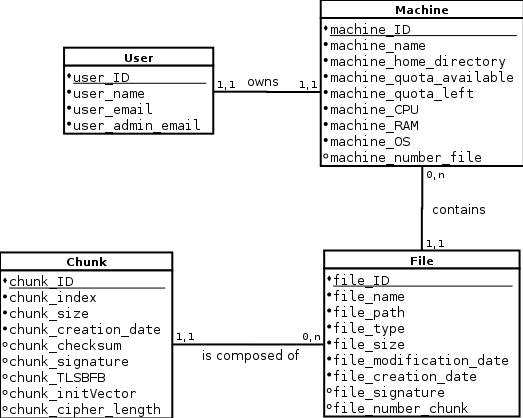
\includegraphics[scale=0.69]{softwareDesign/dbRelClient.png}
  \caption{\label{dbRelClient} Base de donn\'ees relationnelle --- client}
\end{figure}

La signification des diff\'erentes colonnes pr\'esentes figure~\ref{dbRelClient}
se trouve en annexe~\ref{annBDR}.

\paragraph{Choix de la base de donn\'ees}
En plus des m\'eta-donn\'ees des diff\'erents fichiers sauvegard\'es, le
stockage des fichiers sur le serveur a influ\'e sur le choix de la base de
donn\'ees. 

Certaines bases de donn\'ees \textit{NoSQL} offrent la possibilit\'e de 
sauvegarder les fichiers eux-m\^emes. Cela peut \^etre int\'eressant. que ce
soit dans l'imm\'ediat ou dans une future version de l'application.

Donc bien que dans un premier temps nous ayons d\'ecid\'e d'utiliser le
syst\`eme de fichier en place sur le serveur, nous avons pris en compte cette
fonctionnalit\'e.

C'est donc sur \textit{MongoDB} que s'est arr\^et\'e notre choix. Cette base
de donn\'ees a plusieurs avantages qui correspondait \`a ce que nous
recherchions :

\begin{itemize}
 \item R\'eplication automatique des donn\'ees sur plusieurs serveurs
 \item Bonne performance
 \item \textit{GridFS} pour stocker de plus grosses quantit\'es d'information
 (correspondant au fichier sauvegard\'ee dans notre cas).
\end{itemize}

C'est \'egalement une des bases de donn\'ees les plus utilis\'ees pour du
\textit{NoSQL}. La communaut\'e, et donc les sources pour rechercher des
informations relatives \`a son utilisation, est assez importante. N'ayant
jamais utilis\'e \textit{MongoDB} auparavant il \'etait int\'eressant, bien que
pas forc\'ement n\'ecessaire, de pouvoir assez facilement acc\'eder \`a une
possible aide si un probl\`eme arrivait.

Le mod\`ele de stockage dans \textit{MongoDB} est de type documents. La
table~\ref{tabMappSQLMongoTerms} pr\'esente l'\'equivalence entre les termes
utilis\'e pour une base de donn\'ees \textit{SQL} avec ceux utilis\'es dans
\textit{MongoDB}. Plus de pr\'ecisions sont disponible sur le site
\textit{MongoDB}~\cite{refMappingSQLMDB}.

\begin{table}[h!]
  \centering
  \def\arraystretch{1.5}
  \setlength{\fboxsep}{13pt} % padding
  \setlength{\fboxrule}{0pt} % frame
  \begin{tabular}{lm{6cm}m{6cm}}
   \rowcolor{arkred} 
    \arrayrulecolor{gray73}\hline
    \color{white} \textbf{\textit{SQL}} &
    \color{white} \textbf{\textit{MongoDB}}\\
    \hline
    Table & Collection\\
    \hline
    Ligne & Document\\
    \hline
    Colonne & Champ\\
    \hline
    Index & Index\\
    \hline
    Jointure entre tables & Documents int\'egr\'es et li\'es
  \end{tabular}
  \caption{\label{tabMappSQLMongoTerms} \'Equivalent des termes \textit{SQL}
  avec les termes \textit{MongoDB}}
\end{table}

\paragraph{Sch\'emas}
Bien que quelque peu diff\'erent, le sch\'ema des bases de donn\'ees
pr\'esentes sur le serveur et le client ressemble \`a celui pr\'esent
figure~\ref{dbRelClient}.

L'absence de relations entre les diff\'erentes collections a donc oblig\'e une
modification des sch\'emas. De plus, le serveur doit prendre en compte qu'un
utilisateur peut avoir plusieurs machines alors que le client ne s'occupe que
de la machine sur laquelle il est install\'e.

\subparagraph{Client\\}
Les structures suivantes repr\'esentent les collections de la base de donn\'ees
install\'ee sur les machines clientes.

\begin{lstlisting}[language=json]
User :
{ "_id",
  "username",
  "email",
  "admin_email",
  "machine" :
    { "id_machine",
      "name",
      "home_directory",
      "quota_available",
      "quota_left",
      "CPU",
      "RAM",
      "OS"
    }
}
\end{lstlisting}

On voit ici que l'ancienne table \textit{Machine} a \'et\'e int\'egr\'ee dans
la collection \textit{User}. Ce choix s'est fait puisque, sur le client
il n'y a que la machine sur laquelle le logiciel est install\'e qui est
pr\'esente en base de donn\'ees. De plus, l'acc\`es aux donn\'ees est \`a la
fois plus simple et plus rapide en utilisant une collection regroupant
l'utilisateur et sa machine plut\^ot qu'en utilisant deux collections
distinctes.

\begin{lstlisting}[language=json]
File :
{ "_id",
  "filename",
  "filepath",
  "filetype",
  "filesize",
  "modification_date",
  "creation_date",
  "signature",
  "number_chunk"
}
\end{lstlisting}

N'ayant que les informations d'un seul utilisateur et d'une seule machine,
il n'est pas utile de lier d'une quelconque mani\`ere que ce soit la
collection \textit{File} avec la collection \textit{User}.

\begin{lstlisting}[language=json]
Chunk :
{ "_id",
  "id_file"
  "index",
  "size",
  "creation_date",
  "checksum",
  "signature",
  "TLSBFB",
  "init_vector",
  "cipher_length"
}
\end{lstlisting}

Le lien entre la collection \textit{Chunk} et la collection \textit{File} est
repr\'esent\'e par le champ \textit{id\_file} contenant l'identifiant d'un
fichier auquel appartient un morceau.

\subparagraph{Serveur\\}
Bien que similaire, la base de donn\'ees est l\'eg\`erement diff\'erente sur le
serveur par rapport au client. Les changements prennent en compte le fait qu'il
puisse exister plusieurs machines pour un utilisateur mais aussi que plusieurs
utilisateurs existent au sein d'une compagnie.
\begin{lstlisting}[language=json]
User :
{ "_id",
  "id_admin",
  "is_admin",
  "username",
  "email",
  "admin_email",
  "machine" :
    [
      { "id_machine",
	"name",
	"home_directory",
	"quota_available",
	"quota_left",
	"CPU",
	"RAM",
	"OS"
      },
      { "id_machine",
	"name",
	"home_directory",
	"quota_available",
	"quota_left",
	"CPU",
	"RAM",
	"OS"
      },
      ...
    ]
}
\end{lstlisting}
Un utilisateur pouvant avoir plusieurs machines, on cr\'ee simplement une
liste  avec l'ensemble des machines qui est int\'egr\'ee dans la collection
\textit{User}. De plus, un utilisateur pouvant \^etre un administrateur, et
celui-ci pouvant g\'erer plusieurs utilisateurs, on ajoute un lien \`a l'aide
du champ \textit{id\_admin}. Ainsi si le champ n'existe pas, l'utilisateur n'a
pas d'administrateur au-dessus de lui. Aussi \textit{is\_admin} permet de
conna\^itre les privil\`ege d'un utilisateur. L'utilisation de ces deux champs
permet donc de prendre compte qu'un administrateur peut lui-m\^eme avoir un
autre administrateur au-dessus de lui. Cas que l'on peut imaginer possible dans
le cadre de l'utilisation du logiciel au sein d'une grosse soci\'et\'e.

\begin{lstlisting}[language=json]
File :
{ "_id",
  "id_machine",
  "filename",
  "filepath",
  "filetype",
  "filesize",
  "modification_date",
  "creation_date",
  "signature",
  "number_chunk"
}
\end{lstlisting}
Comme plusieurs machines peuvent exister pour un seul utilisateur, on ajoute
le champ \textit{id\_machine} pour pouvoir faire correspondre un fichier \`a
une seule machine.

\begin{lstlisting}[language=json]
Chunk :
{ "_id",
  "id_file"
  "index",
  "size",
  "creation_date",
  "checksum",
  "signature",
  "TLSBFB",
  "init_vector",
  "cipher_length"
}
\end{lstlisting}

\subsubsection{Stockage des fichiers}
Comme nous l'avons vu pr\'ec\'edemment, \textit{MongoDB} combin\'e avec
\textit{GridFS} permet de stocker des fichiers. N\'eanmoins nous avons
d\'ecid\'e d'utiliser, au moins dans un premier temps, le syst\`eme de fichier
disponible sur le serveur : celui-ci ayant de meilleurs performances en lecture
et \'ecriture.

La figure~\ref{fileSystemServer} pr\'esente comment les donn\'ees seront
stock\'ee sur le serveur une fois sauvegard\'ees. Ainsi chaque fichier
correspond \`a un dossier contenant un plusieurs sous-dossier : un par version.
La version d'un fichier correspondant \`a une sauvegarde, un dossier contient
les diff\'erents morceaux sauvegard\'es, c'est-\`a-dire les parties modifi\'ees
du fichier.

\begin{figure}[h!]
  \hspace{-4.5em}
  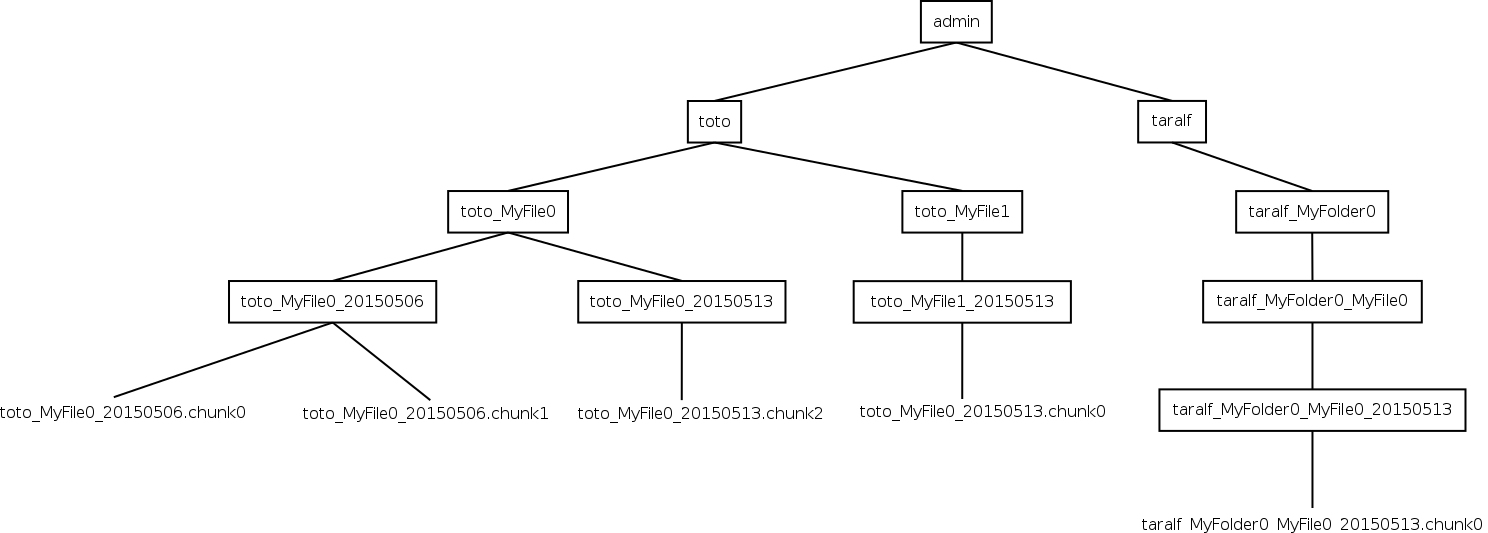
\includegraphics[width=19cm]{softwareDesign/fileSystemServer.png}
  \caption{\label{fileSystemServer} Stockage des fichiers sur le serveur}
\end{figure}

Dans notre exemple, pour r\'ecup\'erer le fichier \textit{MyFile0} de
l'utilisateur \textit{toto}  dans sa version datant du 13 mai 2015, nous devons
donc t\'el\'echarger \textit{toto\_MyFile0\_20150513.chunk2} mais aussi les
morceaux \textit{.chunk0} et \textit{.chunk1} datant de la pr\'ec\'edente
sauvegarde, au 06 mai 2015.

\subsubsection{Communication client - serveur}
Afin d'envoyer les fichiers \`a travers le r\'eseau, un protocole doit \^etre
utilis\'e. Pour ce faire, il m'a \'et\'e demand\'e d'en cr\'eer un correspondant
aux donn\'ees qui sont envoy\'e dans le cadre d'une sauvegarde. En l'occurrence,
les morceaux d'un fichier avec les m\'eta-donn\'ees correspondantes.

Comme indiqu\'e dans la section \flqq~\nameref{secTravailRecherche} \frqq, je me
suis servi du protocole cr\'e\'e pour \textit{syncthings} (\textit{BEP}).
Celui-ci \'etant d\'ecrit sur le github de projet~\cite{refBEP} et
disponible sous licence Creative Commons~\cite{refCC4.0}, il est autoris\'e de
le copier, modifier et r\'eutiliser pour n'importe quelle utilisation, m\^eme
commerciale. Bien que ce dernier point ne nous concerne pas puisque le projet
est doit \^etre Open Source, j'ai pu r\'ecup\'erer le protocole et l'adapter
pour correspondre \`a nos besoins.

Le protocole ainsi modifi\'e est disponible en annexe~\ref{annProtocolComm}, en
anglais puisqu'\'egalement disponible sur le wiki du projet. Celui-ci n'est
n\'eanmoins pas accessible \`a l'heure actuelle puisque le projet est toujours
dans sa phase de d\'eveloppement.


\subsection{D\'eveloppement}
Le client et le serveur \'etant ind\'ependant l'un de l'autre si ce n'est la
partie communication de l'un \`a l'autre, le d\'eveloppement se fait tout
aussi ind\'ependemment.

Le client \'etant la plus grosse partie du syst\`eme de backup, je me suis
concentr\'e sur son d\'eveloppement durant mon stage. Comme il avait \'et\'e
d\'ecoup\'e en module durant la phase de conception, le d\'eveloppement s'est
fait de la m\^eme mani\`ere.

De plus chaque module a le droit \`a sa batterie de test de non r\'egression.

\subsubsection{Outils de d\'eveloppement}
Pour cette phase j'ai utilis\'e plusieurs outils me permettant de construire
au mieux l'application demand\'ee. 

Le d\'eveloppement s'est principalement fait dans un environnement Unix. J'ai
personnellement utilis\'e Debian 7 pour le d\'eveloppement de l'application.
Pouvant avoir acc\`es \`a un environnement Mac OSX dans l'entreprise, j'ai
\'egalement pu tester mon programme sur celui-ci.

La priorit\'e \'etant d'avoir une premi\`ere version fonctionnelle du
programme, je n'ai pas port\'e celui-ci sur un syst\`eme windows durant mon
stage.

\paragraph{Environnement de travail}
\begin{itemize}
 \item \textit{vim} comme \'editeur de texte
 \item \textit{gcc} pour le compilateur
 \item \textit{gdb} pour d\'ebboguer le programme quand n\'ecessaire
 \item \textit{valgrind} pour tout ce qui touche \`a la m\'emoire
 \item \textit{gprof} pour ce qui s'agit de l'analyse de performance
\end{itemize}

\paragraph{Framework et librairies externes}
Afin de limiter les contraintes li\'es \`a l'utilisation de framework et
librairies externes, l'utilisation de ceux-ci \'etait limit\'e. Voici
ceux que j'ai utilis\'e:
\begin{itemize}
 \item \textit{Boost} pour les tests
 \item \textit{OpenSSL} pour tout ce qui est cryptographie
 \item \textit{Magic} pour r\'ecup\'erer des informations sur les fichiers
 comme le MIME type
\end{itemize}

En addition \`a cela, j'ai \'egalement utilis\'e le driver \textit{C++} de
\textit{MongoDB} pour communiquer avec la base de donn\'ees.


\subsubsection{Tests}


\chapter{Rapport technique}
\thispagestyle{fancy}
\label{rapportTechnique}
\section{D\'eroulement du stage}
\subsection{Travail de recherche}
\subsubsection{Prototypage}
Comme expliqu\'e dans le~\nameref{rapportSynthese}, une v\'erification pratique
de la faisabilit\'e de l'algorithme choisi \'etait n\'ecessaire avant de
pouvoir entamer la conception du produit et plusieurs versions ont vu le jour.

\paragraph{Premi\`ere version}



\newpage
\listoffigures
\listoftables
\bibliographystyle{abbrv-fr}
\bibliography{rapport_stage_arksens_2015}

\appendix
\makeatletter
\def\@seccntformat#1{Annexe~\csname the#1\endcsname:\quad}
\makeatother
\chapter{Base de donn\'ees relationnelle}
\label{annBDR}
\thispagestyle{fancy}
\section{User}
\begin{table}[h!]
  \centering
  \def\arraystretch{1.5}
  \setlength{\fboxsep}{13pt} % padding
  \setlength{\fboxrule}{0pt} % frame
  \begin{tabular}{lm{6cm}m{6cm}}
   \rowcolor{arkred} 
    \arrayrulecolor{gray73}\hline
    \color{white} \textbf{Colonne} & \color{white} \textbf{Information}\\
    \hline
    user\_id & Identifiant unique pour l'utilisateur\\
    \hline
    user\_name & Nom de l'utilisateur\\
    \hline
    user\_email & Email de l'utilisateur\\
    \hline
    user\_admin\_email & Email de l'administrateur en charge de l'utilisateur.
    Utilis\'e pour pr\'evenir automatiquement l'administrateur en cas de
    probl\`eme de fonctionnement.
  \end{tabular}
  \caption{\label{tabDBRUser} Information colonnes -- User}
\end{table}

\section{Machine}
\begin{table}[h!]
  \centering
  \def\arraystretch{1.5}
  \setlength{\fboxsep}{13pt} % padding
  \setlength{\fboxrule}{0pt} % frame
  \begin{tabular}{lm{6cm}m{6cm}}
   \rowcolor{arkred} 
    \arrayrulecolor{gray73}\hline
    \color{white} \textbf{Colonne} & \color{white} \textbf{Information}\\
    \hline
    machine\_id & Identifiant unique pour la machine\\
    \hline
    machine\_name & Nom de la machine\\
    \hline
    machine\_home\_directory & R\'epertoire racine des fichiers \`a sauvegarder\\
    \hline
    machine\_quota\_available & Quota disponible (total) pour la machine\\
    \hline
    machine\_quota\_left & Quota restant pour la machine\\
    \hline
    machine\_CPU & Informations relatives au processeur utilis\'e\\
    \hline
    machine\_RAM & Quantit\'e de RAM disponible\\
    \hline
    machine\_OS & Syst\`eme d'exploitation utilis\'e\\
    \hline
    machine\_number\_file & Nombre de fichier sauvegard\'e
  \end{tabular}
  \caption{\label{tabDBRMachine} Information colonnes -- Machine}
\end{table}

\section{File}
\begin{table}[h!]
  \centering
  \def\arraystretch{1.5}
  \setlength{\fboxsep}{13pt} % padding
  \setlength{\fboxrule}{0pt} % frame
  \begin{tabular}{lm{6cm}m{6cm}}
   \rowcolor{arkred} 
    \arrayrulecolor{gray73}\hline
    \color{white} \textbf{Colonne} & \color{white} \textbf{Information}\\
    \hline
    file\_id & Identifiant unique du fichier\\
    \hline
    file\_name & Nom du fichier\\
    \hline
    file\_path & Chemin du fichier en local\\
    \hline
    file\_type & Type du fichier\\
    \hline
    file\_size & Taille du fichier en octet\\
    \hline
    file\_modification\_date & Date de derni\`ere modification\\
    \hline
    file\_creation\_date & Date de cr\'eation\\
    \hline
    file\_signature & Signature num\'erique\\
    \hline
    file\_number\_chunk & Nombre de morceau composant le fichier
  \end{tabular}
  \caption{\label{tabDBRMachine} Information colonnes -- File}
\end{table}

\section{Chunk}
\begin{savenotes}
\begin{table}[h!]
  \centering
  \def\arraystretch{1.5}
  \setlength{\fboxsep}{13pt} % padding
  \setlength{\fboxrule}{0pt} % frame
  \begin{tabular}{lm{6cm}m{6cm}}
   \rowcolor{arkred} 
    \arrayrulecolor{gray73}\hline
    \color{white} \textbf{Colonne} & \color{white} \textbf{Information}\\
    \hline
    chunk\_id & Identifiant unique d'un morceau de fichier\\
    \hline
    chunk\_index & Index du morceau de fichier\\
    \hline
    chunk\_size & Taille du morceau en octet\\
    \hline
    chunk\_creation\_date & Date de cr\'eation\\
    \hline
    chunk\_checksum & Checksum\\
    \hline
    chunk\_signature & Signature num\'erique\\
    \hline
    chunk\_TLSBFB\footnote{Two Last Significant Bit of First Byte} & Deux bits
    de poids faible du premier octet du morceau. Utilis\'e pour r\'epartir le
    travail entre plusieurs thread lors du scan d'un fichier pour trouver les
    parties modifi\'es de celui-ci.\\
    \hline
    chunk\_init\_vector & Vecteur d'initialisation utilis\'e pour l'algorithme de
    chiffrement AES\\
    \hline
    chunk\_cipher\_length & Taille du morceau chiffr\'e en octet\\
  \end{tabular}
  \caption{\label{tabDBRMachine} Information colonnes -- Chunk}
\end{table}
\end{savenotes}


\chapter{Protocole de communication}
\label{annProtocolComm}
\thispagestyle{fancy}
\section{Definition}

The key words "MUST", "MUST NOT", "REQUIRED", "SHALL", "SHALL NOT",
"SHOULD", "SHOULD NOT", "RECOMMENDED", "MAY", and "OPTIONAL" in this
document are to be interpreted as described in RFC 2119.


\section{Transport and Authentication}

This protocol is deployed as the highest level in a protocol stack, with
the lower level protocols providing additional encryption and authentication.

\begin{verbatim}
           +-----------------------------|
           |   Block Exchange Protocol   |
           |-----------------------------|
           | Encryption & Auth (TLS 1.2) |
           |-----------------------------|
           |             TCP             |
           |-----------------------------|
           v             ...             v
\end{verbatim}

\section{Messages}

Every message starts with one 32 bit word indicating the message version,
type and ID, followed by the length of the message. The header is in
network byte order, i.e. big endian.

\begin{itemize}
 \item Message Structure:
\end{itemize}

\begin{verbatim}
            O                   1                   2                   3
            O 1 2 3 4 5 6 7 8 9 0 1 2 3 4 5 6 7 8 9 0 1 2 3 4 5 6 7 8 9 0 1
           +-+-+-+-+-+-+-+-+-+-+-+-+-+-+-+-+-+-+-+-+-+-+-+-+-+-+-+-+-+-+-+-+
           |  Ver  |       Message ID      |      Type     |    Reserved   |
           +-+-+-+-+-+-+-+-+-+-+-+-+-+-+-+-+-+-+-+-+-+-+-+-+-+-+-+-+-+-+-+-+
           |                            Length                             |
           +-+-+-+-+-+-+-+-+-+-+-+-+-+-+-+-+-+-+-+-+-+-+-+-+-+-+-+-+-+-+-+-+
\end{verbatim}

For version 1 the Version field is set to zero. Future versions with
incompatible message formats will increment the Version field. A
message with an unknown version is a protocol error and MUST result
in the connection being terminated. A client supporting multiple
versions MAY retry with a different protocol version upon disconnection.

The Message ID is set to a unique value for each transmitted request
message. In response messages it is set to the Message ID of the
corresponding request message. The uniqueness requirement implies that
no more than 4096 messages may be outstanding at any given moment. The
ordering requirement implies that a response to a given message ID also
means that all preceding messages have been received, specifically
those which do not otherwise demand a response. Hence their message
ID:s may be reused.

The Type field indicates the type of data following the message header
and is one of the integers defined below. A message of an unknown type
is a protocol error and MUST result in the connection being terminated.


\section{Types}
\subsection{0 - Client Config}

This informational message provides information about the client
configuration as it pertains to the current connection. A Client
Config message MUST be the first message sent on a connection.
Additional Client Config messages MUST NOT be sent after the initial
exchange.

\begin{itemize}
 \item ClientConfigMessage Structure:
\end{itemize}

\begin{verbatim}
            O                   1                   2                   3
            O 1 2 3 4 5 6 7 8 9 0 1 2 3 4 5 6 7 8 9 0 1 2 3 4 5 6 7 8 9 0 1
           +-+-+-+-+-+-+-+-+-+-+-+-+-+-+-+-+-+-+-+-+-+-+-+-+-+-+-+-+-+-+-+-+
           |                     Length of ClientName                      |
           +-+-+-+-+-+-+-+-+-+-+-+-+-+-+-+-+-+-+-+-+-+-+-+-+-+-+-+-+-+-+-+-+
           /                                                               /
           \                 ClientName (variable length)                  \
           /                                                               /
           +-+-+-+-+-+-+-+-+-+-+-+-+-+-+-+-+-+-+-+-+-+-+-+-+-+-+-+-+-+-+-+-+
           |                    Length of ClientVersion                    |
           +-+-+-+-+-+-+-+-+-+-+-+-+-+-+-+-+-+-+-+-+-+-+-+-+-+-+-+-+-+-+-+-+
           /                                                               /
           \                ClientVersion (variable length)                \
           /                                                               /
           +-+-+-+-+-+-+-+-+-+-+-+-+-+-+-+-+-+-+-+-+-+-+-+-+-+-+-+-+-+-+-+-+
           |                       Number of Folders                       |
           +-+-+-+-+-+-+-+-+-+-+-+-+-+-+-+-+-+-+-+-+-+-+-+-+-+-+-+-+-+-+-+-+
           /                                                               /
           \                Zero or more Folder Structures                 \
           /                                                               /
           +-+-+-+-+-+-+-+-+-+-+-+-+-+-+-+-+-+-+-+-+-+-+-+-+-+-+-+-+-+-+-+-+
           |                       Number of Options                       |
           +-+-+-+-+-+-+-+-+-+-+-+-+-+-+-+-+-+-+-+-+-+-+-+-+-+-+-+-+-+-+-+-+
           /                                                               /
           \                Zero or more Option Structures                 \
           /                                                               /
           +-+-+-+-+-+-+-+-+-+-+-+-+-+-+-+-+-+-+-+-+-+-+-+-+-+-+-+-+-+-+-+-+
\end{verbatim}

\begin{itemize}
 \item Folder Structure:
\end{itemize}

\begin{verbatim}
            O                   1                   2                   3
            O 1 2 3 4 5 6 7 8 9 0 1 2 3 4 5 6 7 8 9 0 1 2 3 4 5 6 7 8 9 0 1
           +-+-+-+-+-+-+-+-+-+-+-+-+-+-+-+-+-+-+-+-+-+-+-+-+-+-+-+-+-+-+-+-+
           |                         Length of ID                          |
           +-+-+-+-+-+-+-+-+-+-+-+-+-+-+-+-+-+-+-+-+-+-+-+-+-+-+-+-+-+-+-+-+
           /                                                               /
           \                     ID (variable length)                      \
           /                                                               /
           +-+-+-+-+-+-+-+-+-+-+-+-+-+-+-+-+-+-+-+-+-+-+-+-+-+-+-+-+-+-+-+-+
           |                       Number of Folders                       |
           +-+-+-+-+-+-+-+-+-+-+-+-+-+-+-+-+-+-+-+-+-+-+-+-+-+-+-+-+-+-+-+-+
           /                                                               /
           \                Zero or more Folder Structures                 \
           /                                                               /
           +-+-+-+-+-+-+-+-+-+-+-+-+-+-+-+-+-+-+-+-+-+-+-+-+-+-+-+-+-+-+-+-+
\end{verbatim}

\begin{itemize}
 \item Option Structure:
\end{itemize}

\begin{verbatim}
            O                   1                   2                   3
            O 1 2 3 4 5 6 7 8 9 0 1 2 3 4 5 6 7 8 9 0 1 2 3 4 5 6 7 8 9 0 1
           +-+-+-+-+-+-+-+-+-+-+-+-+-+-+-+-+-+-+-+-+-+-+-+-+-+-+-+-+-+-+-+-+
           |                         Length of Key                         |
           +-+-+-+-+-+-+-+-+-+-+-+-+-+-+-+-+-+-+-+-+-+-+-+-+-+-+-+-+-+-+-+-+
           /                                                               /
           \                     Key (variable length)                     \
           /                                                               /
           +-+-+-+-+-+-+-+-+-+-+-+-+-+-+-+-+-+-+-+-+-+-+-+-+-+-+-+-+-+-+-+-+
           |                        Length of Value                        |
           +-+-+-+-+-+-+-+-+-+-+-+-+-+-+-+-+-+-+-+-+-+-+-+-+-+-+-+-+-+-+-+-+
           /                                                               /
           \                    Value (variable length)                    \
           /                                                               /
           +-+-+-+-+-+-+-+-+-+-+-+-+-+-+-+-+-+-+-+-+-+-+-+-+-+-+-+-+-+-+-+-+
\end{verbatim}

The ClientName and ClientVersion fields identify the implementation.
The values SHOULD be simple strings identifying the implementation name,
as a user would expect to see it, and the version string in the same
manner. An example ClientName is "acs" and an example ClientVersion is
"v0.7.2". The ClientVersion field SHOULD follow the patterns laid out
in the [Semantic Versioning](http://semver.org/) standard.

The Folders field lists all folders that will be synchronized over the
current connection. Each folder has a list of sub-folders.

The Options field contain option values to be used in an implementation
specific manner. The options list is conceptually a map of Key => Value
items, although it is transmitted in the form of a list of (Key, Value)
pairs, both of string type. Key ID:s are implementation specific. An
implementation MUST ignore unknown keys. An implementation MAY impose
limits on the length keys and values. The options list may be used to
inform of relevant information such as quota and other user information
for example.

\subsection{1 - Index \&\& 7 - Index Update}

This TypeMessages will be used for Client -> Server communication,
i.e.~the actual backup.

The Index and Index Update messages define the contents of the senders
folder. An Index message represents the full contents of the folder and
thus supersedes any previous index. An Index Update amends an existing
index with new information, not affecting any entries not included in
the message.

An Index or Index Update message MUST be sent for each folder included
in the Client Config message, and MUST be sent before any other message
referring to that folder. If the folder contents change from non-empty
to empty, an empty Index message MUST be sent. There is no response to
the Index message.

\begin{itemize}
 \item IndexMessage Structure: 
\end{itemize}

\begin{verbatim}
            O                   1                   2                   3
            O 1 2 3 4 5 6 7 8 9 0 1 2 3 4 5 6 7 8 9 0 1 2 3 4 5 6 7 8 9 0 1
           +-+-+-+-+-+-+-+-+-+-+-+-+-+-+-+-+-+-+-+-+-+-+-+-+-+-+-+-+-+-+-+-+
           |                       Length of Folder                        |
           +-+-+-+-+-+-+-+-+-+-+-+-+-+-+-+-+-+-+-+-+-+-+-+-+-+-+-+-+-+-+-+-+
           /                                                               /
           \                   Folder (variable length)                    \
           /                                                               /
           +-+-+-+-+-+-+-+-+-+-+-+-+-+-+-+-+-+-+-+-+-+-+-+-+-+-+-+-+-+-+-+-+
           |                        Number of Files                        |
           +-+-+-+-+-+-+-+-+-+-+-+-+-+-+-+-+-+-+-+-+-+-+-+-+-+-+-+-+-+-+-+-+
           /                                                               /
           \               Zero or more FileInfo Structures                \
           /                                                               /
           +-+-+-+-+-+-+-+-+-+-+-+-+-+-+-+-+-+-+-+-+-+-+-+-+-+-+-+-+-+-+-+-+
\end{verbatim}

\begin{itemize}
 \item FileInfo Structure:
\end{itemize}

\begin{verbatim}
            O                   1                   2                   3
            O 1 2 3 4 5 6 7 8 9 0 1 2 3 4 5 6 7 8 9 0 1 2 3 4 5 6 7 8 9 0 1
           +-+-+-+-+-+-+-+-+-+-+-+-+-+-+-+-+-+-+-+-+-+-+-+-+-+-+-+-+-+-+-+-+
           |                         Length of ID                          |
           +-+-+-+-+-+-+-+-+-+-+-+-+-+-+-+-+-+-+-+-+-+-+-+-+-+-+-+-+-+-+-+-+
           /                                                               /
           \                     ID (variable length)                      \
           /                                                               /
           +-+-+-+-+-+-+-+-+-+-+-+-+-+-+-+-+-+-+-+-+-+-+-+-+-+-+-+-+-+-+-+-+
           |                        Length of Name                         |
           +-+-+-+-+-+-+-+-+-+-+-+-+-+-+-+-+-+-+-+-+-+-+-+-+-+-+-+-+-+-+-+-+
           /                                                               /
           \                    Name (variable length)                     \
           /                                                               /
           +-+-+-+-+-+-+-+-+-+-+-+-+-+-+-+-+-+-+-+-+-+-+-+-+-+-+-+-+-+-+-+-+
           |                                                               |
           +                      Modified (64 bits)                       +
           |                                                               |
           +-+-+-+-+-+-+-+-+-+-+-+-+-+-+-+-+-+-+-+-+-+-+-+-+-+-+-+-+-+-+-+-+
           |                       Number of Blocks                        |
           +-+-+-+-+-+-+-+-+-+-+-+-+-+-+-+-+-+-+-+-+-+-+-+-+-+-+-+-+-+-+-+-+
           /                                                               /
           \               Zero or more BlockInfo Structures               \
           /                                                               /
           +-+-+-+-+-+-+-+-+-+-+-+-+-+-+-+-+-+-+-+-+-+-+-+-+-+-+-+-+-+-+-+-+
\end{verbatim}

\begin{itemize}
 \item BlockInfo Structure:
\end{itemize}

\begin{verbatim}
            O                   1                   2                   3
            O 1 2 3 4 5 6 7 8 9 0 1 2 3 4 5 6 7 8 9 0 1 2 3 4 5 6 7 8 9 0 1
           +-+-+-+-+-+-+-+-+-+-+-+-+-+-+-+-+-+-+-+-+-+-+-+-+-+-+-+-+-+-+-+-+
           |                             Size                              |
           +-+-+-+-+-+-+-+-+-+-+-+-+-+-+-+-+-+-+-+-+-+-+-+-+-+-+-+-+-+-+-+-+
           |lsb|                        Reserved                           |
           +-+-+-+-+-+-+-+-+-+-+-+-+-+-+-+-+-+-+-+-+-+-+-+-+-+-+-+-+-+-+-+-+
           |                      Length of Signature                      |
           +-+-+-+-+-+-+-+-+-+-+-+-+-+-+-+-+-+-+-+-+-+-+-+-+-+-+-+-+-+-+-+-+
           /                                                               /
           \                  Signature (variable length)                  \
           /                                                               /
           +-+-+-+-+-+-+-+-+-+-+-+-+-+-+-+-+-+-+-+-+-+-+-+-+-+-+-+-+-+-+-+-+
           |                      Length of Checksum                       |
           +-+-+-+-+-+-+-+-+-+-+-+-+-+-+-+-+-+-+-+-+-+-+-+-+-+-+-+-+-+-+-+-+
           /                                                               /
           \                   Checksum (variable length)                  \
           /                                                               /
           +-+-+-+-+-+-+-+-+-+-+-+-+-+-+-+-+-+-+-+-+-+-+-+-+-+-+-+-+-+-+-+-+
           |                          Block Index                          |
           +-+-+-+-+-+-+-+-+-+-+-+-+-+-+-+-+-+-+-+-+-+-+-+-+-+-+-+-+-+-+-+-+
           |                        Length of Data                         |
           +-+-+-+-+-+-+-+-+-+-+-+-+-+-+-+-+-+-+-+-+-+-+-+-+-+-+-+-+-+-+-+-+
           /                                                               /
           \                    Data (variable length)                     \
           /                                                               /
           +-+-+-+-+-+-+-+-+-+-+-+-+-+-+-+-+-+-+-+-+-+-+-+-+-+-+-+-+-+-+-+-+
\end{verbatim}

The Folder field identifies the folder that the index message pertains
to.

The Name is the file name path relative to the folder root. Like all
strings, the Name is always in UTF-8 NFC regardless of operating system
or file system specific conventions. The Name field uses the slash
character ("/") as path separator, regardless of the implementation's
operating system conventions. The combination of Folder and Name
identifies each file on a Client machine as well as a unique ID
specified by Adhara.

The Modified time is expressed as the number of seconds since the Unix
Epoch (1970-01-01 00:00:00 UTC).

The Blocks list contains the size, signature, checksum, block index
and the two least significant bit of the first byte of the block (lsb)
for each block in the file.

\subsection{2 - Request}

The Request message expresses the desire to retrieve a file from the
server or to get the data on modified files to synchronize.

\begin{itemize}
 \item RequestMessage Structure:
\end{itemize}

\begin{verbatim}
            O                   1                   2                   3
            O 1 2 3 4 5 6 7 8 9 0 1 2 3 4 5 6 7 8 9 0 1 2 3 4 5 6 7 8 9 0 1
           +-+-+-+-+-+-+-+-+-+-+-+-+-+-+-+-+-+-+-+-+-+-+-+-+-+-+-+-+-+-+-+-+
           |                       Length of Folder                        |
           +-+-+-+-+-+-+-+-+-+-+-+-+-+-+-+-+-+-+-+-+-+-+-+-+-+-+-+-+-+-+-+-+
           /                                                               /
           \                   Folder (variable length)                    \
           /                                                               /
           +-+-+-+-+-+-+-+-+-+-+-+-+-+-+-+-+-+-+-+-+-+-+-+-+-+-+-+-+-+-+-+-+
           |                        Length of Name                         |
           +-+-+-+-+-+-+-+-+-+-+-+-+-+-+-+-+-+-+-+-+-+-+-+-+-+-+-+-+-+-+-+-+
           /                                                               /
           \                    Name (variable length)                     \
           /                                                               /
           +-+-+-+-+-+-+-+-+-+-+-+-+-+-+-+-+-+-+-+-+-+-+-+-+-+-+-+-+-+-+-+-+
           |                             Size                              |
           +-+-+-+-+-+-+-+-+-+-+-+-+-+-+-+-+-+-+-+-+-+-+-+-+-+-+-+-+-+-+-+-+
           |                      Length of Signature                      |
           +-+-+-+-+-+-+-+-+-+-+-+-+-+-+-+-+-+-+-+-+-+-+-+-+-+-+-+-+-+-+-+-+
           /                                                               /
           \                  Signature (variable length)                  \
           /                                                               /
           +-+-+-+-+-+-+-+-+-+-+-+-+-+-+-+-+-+-+-+-+-+-+-+-+-+-+-+-+-+-+-+-+
           |      Type     |                  Reserved                     |
           +-+-+-+-+-+-+-+-+-+-+-+-+-+-+-+-+-+-+-+-+-+-+-+-+-+-+-+-+-+-+-+-+
\end{verbatim}

The size and signature field MAY be set to the expected size and
signature values of the block, or may be left empty (zero length).
If set, the server SHOULD ensure that the transmitted block matches
the requested size and signature.

Type corresponds to the expected type of the reply:
\begin{itemize}
 \item 3 - ResponseData
 \item 4 - ResponseFileInfo
\end{itemize}

\subsection{3 - ResponseData}

The ResponseData message is sent in response to a Request message.

\begin{itemize}
 \item ResponseDataMessage Structure:
\end{itemize}

\begin{verbatim}
            O                   1                   2                   3
            O 1 2 3 4 5 6 7 8 9 0 1 2 3 4 5 6 7 8 9 0 1 2 3 4 5 6 7 8 9 0 1
           +-+-+-+-+-+-+-+-+-+-+-+-+-+-+-+-+-+-+-+-+-+-+-+-+-+-+-+-+-+-+-+-+
           |                        Length of Data                         |
           +-+-+-+-+-+-+-+-+-+-+-+-+-+-+-+-+-+-+-+-+-+-+-+-+-+-+-+-+-+-+-+-+
           /                                                               /
           \                    Data (variable length)                     \
           /                                                               /
           +-+-+-+-+-+-+-+-+-+-+-+-+-+-+-+-+-+-+-+-+-+-+-+-+-+-+-+-+-+-+-+-+
           |                             Code                              |
           +-+-+-+-+-+-+-+-+-+-+-+-+-+-+-+-+-+-+-+-+-+-+-+-+-+-+-+-+-+-+-+-+
\end{verbatim}

The Code field contains an error code describing the reason a Request
could not be fulfilled, in the case where a zero length Data was
returned. The following values are defined:


\begin{itemize}
 \item 0: No Error (Data should be present)
 \item 1: Generic Error
 \item 2: No Such File (the requested file does not exist, or the offset is
  outside the acceptable range for the file)
 \item 3: Invalid (file exists but has invalid bit set or is otherwise
  unavailable)
\end{itemize}

\subsection{4 - ReponseFileInfo}

The ResponseFileInfo is sent in response to a Request message.

\begin{itemize}
 \item ResponseFileInfoMessage Structure:
\end{itemize}

\begin{verbatim}
            O                   1                   2                   3
            O 1 2 3 4 5 6 7 8 9 0 1 2 3 4 5 6 7 8 9 0 1 2 3 4 5 6 7 8 9 0 1
           +-+-+-+-+-+-+-+-+-+-+-+-+-+-+-+-+-+-+-+-+-+-+-+-+-+-+-+-+-+-+-+-+
           |                             Size                              |
           +-+-+-+-+-+-+-+-+-+-+-+-+-+-+-+-+-+-+-+-+-+-+-+-+-+-+-+-+-+-+-+-+
           |                      Length of Signature                      |
           +-+-+-+-+-+-+-+-+-+-+-+-+-+-+-+-+-+-+-+-+-+-+-+-+-+-+-+-+-+-+-+-+
           /                                                               /
           \                  Signature (variable length)                  \
           /                                                               /
           +-+-+-+-+-+-+-+-+-+-+-+-+-+-+-+-+-+-+-+-+-+-+-+-+-+-+-+-+-+-+-+-+
           |                      Length of Checksum                       |
           +-+-+-+-+-+-+-+-+-+-+-+-+-+-+-+-+-+-+-+-+-+-+-+-+-+-+-+-+-+-+-+-+
           /                                                               /
           \                   Checksum (variable length)                  \
           /                                                               /
           +-+-+-+-+-+-+-+-+-+-+-+-+-+-+-+-+-+-+-+-+-+-+-+-+-+-+-+-+-+-+-+-+
           |                       Number of Blocks                        |
           +-+-+-+-+-+-+-+-+-+-+-+-+-+-+-+-+-+-+-+-+-+-+-+-+-+-+-+-+-+-+-+-+
           /                                                               /
           \               Zero or more BlockInfo Structures               \
           /                                                               /
           +-+-+-+-+-+-+-+-+-+-+-+-+-+-+-+-+-+-+-+-+-+-+-+-+-+-+-+-+-+-+-+-+
           |                             Code                              |
           +-+-+-+-+-+-+-+-+-+-+-+-+-+-+-+-+-+-+-+-+-+-+-+-+-+-+-+-+-+-+-+-+
\end{verbatim}

\begin{itemize}
  \item BlockInfo Structure:
\end{itemize}

\begin{verbatim}
            O                   1                   2                   3
            O 1 2 3 4 5 6 7 8 9 0 1 2 3 4 5 6 7 8 9 0 1 2 3 4 5 6 7 8 9 0 1
           +-+-+-+-+-+-+-+-+-+-+-+-+-+-+-+-+-+-+-+-+-+-+-+-+-+-+-+-+-+-+-+-+
           |                             Size                              |
           +-+-+-+-+-+-+-+-+-+-+-+-+-+-+-+-+-+-+-+-+-+-+-+-+-+-+-+-+-+-+-+-+
           |lsb|                        Reserved                           |
           +-+-+-+-+-+-+-+-+-+-+-+-+-+-+-+-+-+-+-+-+-+-+-+-+-+-+-+-+-+-+-+-+
           |                      Length of Signature                      |
           +-+-+-+-+-+-+-+-+-+-+-+-+-+-+-+-+-+-+-+-+-+-+-+-+-+-+-+-+-+-+-+-+
           /                                                               /
           \                  Signature (variable length)                  \
           /                                                               /
           +-+-+-+-+-+-+-+-+-+-+-+-+-+-+-+-+-+-+-+-+-+-+-+-+-+-+-+-+-+-+-+-+
           |                      Length of Checksum                       |
           +-+-+-+-+-+-+-+-+-+-+-+-+-+-+-+-+-+-+-+-+-+-+-+-+-+-+-+-+-+-+-+-+
           /                                                               /
           \                   Checksum (variable length)                  \
           /                                                               /
           +-+-+-+-+-+-+-+-+-+-+-+-+-+-+-+-+-+-+-+-+-+-+-+-+-+-+-+-+-+-+-+-+
           |                          Block Index                          |
           -+-+-+-+-+-+-+-+-+-+-+-+-+-+-+-+-+-+-+-+-+-+-+-+-+-+-+-+-+-+-+-+
           |                        Length of Data                         |
           +-+-+-+-+-+-+-+-+-+-+-+-+-+-+-+-+-+-+-+-+-+-+-+-+-+-+-+-+-+-+-+-+
           /                                                               /
           \                    Data (variable length)                     \
           /                                                               /
           +-+-+-+-+-+-+-+-+-+-+-+-+-+-+-+-+-+-+-+-+-+-+-+-+-+-+-+-+-+-+-+-+
           |                             Code                              |
           +-+-+-+-+-+-+-+-+-+-+-+-+-+-+-+-+-+-+-+-+-+-+-+-+-+-+-+-+-+-+-+-+
\end{verbatim}

The different fields are defined as they were previously.


\subsection{5 - Ping}
No content. The Ping message is used to determine that a connection is
alive.

\subsection{6 - Pong}
No content but copies the Message ID from the Ping.

\subsection{8 - Close}

The Close message MAY be sent to indicate that the connection will be
torn down due to an error condition. A Close message MUST NOT be
followed by further messages.

\begin{itemize}
 \item CloseMessage Structure: 
\end{itemize}
 
\begin{verbatim}
            O                   1                   2                   3
            O 1 2 3 4 5 6 7 8 9 0 1 2 3 4 5 6 7 8 9 0 1 2 3 4 5 6 7 8 9 0 1
           +-+-+-+-+-+-+-+-+-+-+-+-+-+-+-+-+-+-+-+-+-+-+-+-+-+-+-+-+-+-+-+-+
           |                       Length of Reason                        |
           +-+-+-+-+-+-+-+-+-+-+-+-+-+-+-+-+-+-+-+-+-+-+-+-+-+-+-+-+-+-+-+-+
           /                                                               /
           \                   Reason (variable length)                    \
           /                                                               /
           +-+-+-+-+-+-+-+-+-+-+-+-+-+-+-+-+-+-+-+-+-+-+-+-+-+-+-+-+-+-+-+-+
           |                             Code                              |
           +-+-+-+-+-+-+-+-+-+-+-+-+-+-+-+-+-+-+-+-+-+-+-+-+-+-+-+-+-+-+-+-+
\end{verbatim}


The Reason field contains a human description of the error condition,
suitable for consumption by a human. The Code field is for a machine
readable error code.

\end{spacing}
\end{document}          